\chapter{Présentation de mon activité}
	\section{\adt{} V7}	
	Durant ce stage, j'ai travaillé sur le produit \adt{} qui est actuellement en version V7.

	\adt{} est une plateforme complète de TEM\footnote{Telecom Expense Management} particulièrement adaptée au contexte des Grands Comptes.  Elle équipe également des fournisseurs de services soucieux d’apporter à leurs clients des solutions éprouvées à forte valeur ajoutée.  Entièrement modulaire, elle s’adapte aux souhaits et aux contraintes des clients et permet de gérer l’ensemble du budget et des ressources télécoms : voix, data fixes et mobiles.

\begin{figure}[H]
	\centering
	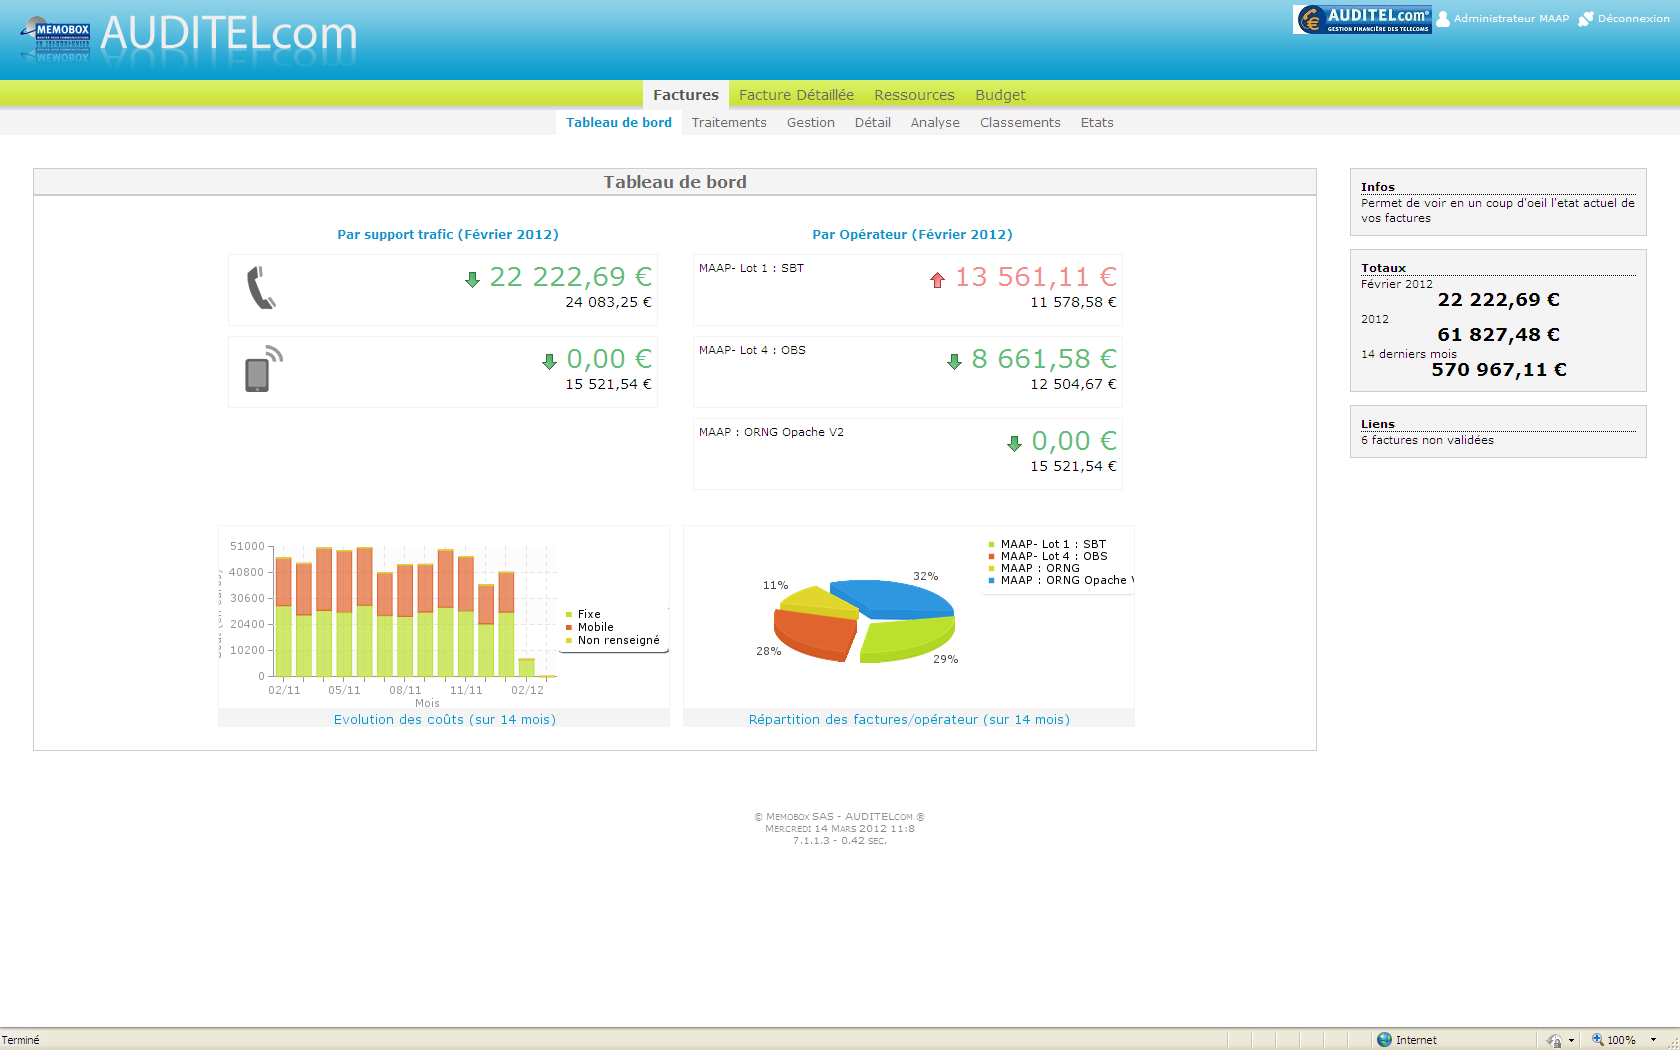
\includegraphics[width=12cm]{images/2-activite/screenAdt.png}
	\caption{\adt{} V7}
\end{figure}
\adt{} est un service en ligne qui, de part son architecture modulaire et sa forte industrialisation, s’adresse aussi bien aux PME\footnote{Petites et Moyennes Entreprises} qu’aux Grands Comptes et Très Grands Comptes.

Fonctionnant en mode SaaS\footnote{Software as a Service}, Cette plateforme peut être installée chez un client ou mutualisée dans les locaux d’un fournisseur de services ou dans ceux de \mbx{}.

Elle assure une qualité irréprochable des données, chose essentielle pour une solution de TEM :
\begin{itemize}
\item Les grilles tarifaires des opérateurs sont en permanence à jour,
\item Les nouveaux PABX et IPBX sont toujours pris en compte,
\item Les nouvelles fonctions statistiques sont mise en ligne,
\item Les nouvelles fonctionnalités sont automatiquement activées.
\end{itemize}


L’offre de service \adt{} délivrée sous forme d’un abonnement, est une solution clé en main permettant de ne pas investir en matériel et logiciel, et de ne pas monopoliser de ressources et de compétences particulières.


\section{Mon rôle}
Lors de mon stage, j'ai participé au développement de \adt{}. J'ai intégré l'équipe de développement composée de \Romain{} et \Denis{}, le système étant en production, il fallait faire attention à n'effectuer aucune régression de l'application,
et effectuer suffisamment de tests avant que mes modifications ne soient apportées sur le serveur de production afin que les clients ne subissent aucune préjudice.

Le développement d'\adt{} fut commencé dans les années 2000 et plusieurs développeurs ont apporté leur contribution, ainsi, on pouvait distinguer différents styles de programmation, certaines portions de code pouvant être vieillissantes.

Lors de mon arrivée, \adt{} était destiné à être multilingue, ainsi il était possible de se connecter en Français, Anglais ou Espagnol. Cependant le système qui permettait à l'application d'être multilingue n'était pas parfait, et rendait difficile la maintenance et
la traduction de l'application. En effet, lorsque nous nous connections pour visualiser l'application en Anglais, la traduction n'était pas effective partout. Ainsi, certaines phrases s'affichaient en français. Cependant la traduction n'allait pas continuer tant que le système n'était pas viable.

Ainsi, mon travail fut d'étudier le système déjà développé, afin d'en analyser les erreurs qui ont été faites pour pouvoir concevoir un nouveau système qui serait beaucoup plus stable et pérenne et rendrait le travail de traduction le plus simple et rapide possible.


\section{\'Etude de l'existant}
\subsection{Le système}
Pour son système de traduction l'application possédait une classe \texttt{TTranslator}, toutes les traductions devaient passer via cette classe à l'aide d'un singleton, la classe \texttt{TTranslator} faisait ensuite des appels à la classe \texttt{TDataLinkAbstract} pour faire le lien
avec la base de données contenant toutes les traductions.
\subsubsection{La table \texttt{RES\_Translations} dite Ancienne Table}
Toutes les traductions étaient stockées dans la table \texttt{RES\_Translations}, ci-dessous sa structure.
\begin{figure}[H]
\centering
% Graphic for TeX using PGF
% Title: C:\Documents and Settings\antoine.deroquemaure\Mes documents\rapportStage\rapport\images\2-activite\bdExistant.dia
% Creator: Dia v0.97.2
% CreationDate: Tue May 29 16:48:55 2012
% For: antoine.deroquemaure
% \usepackage{tikz}
% The following commands are not supported in PSTricks at present
% We define them conditionally, so when they are implemented,
% this pgf file will use them.
\ifx\du\undefined
  \newlength{\du}
\fi
\setlength{\du}{15\unitlength}
\begin{tikzpicture}
\pgftransformxscale{1.000000}
\pgftransformyscale{-1.000000}
\definecolor{dialinecolor}{rgb}{0.000000, 0.000000, 0.000000}
\pgfsetstrokecolor{dialinecolor}
\definecolor{dialinecolor}{rgb}{1.000000, 1.000000, 1.000000}
\pgfsetfillcolor{dialinecolor}
\pgfsetlinewidth{0.030000\du}
\pgfsetdash{}{0pt}
\definecolor{dialinecolor}{rgb}{1.000000, 1.000000, 1.000000}
\pgfsetfillcolor{dialinecolor}
\fill (17.850000\du,14.900000\du)--(17.850000\du,16.300000\du)--(27.205000\du,16.300000\du)--(27.205000\du,14.900000\du)--cycle;
\definecolor{dialinecolor}{rgb}{0.000000, 0.000000, 0.000000}
\pgfsetstrokecolor{dialinecolor}
\draw (17.850000\du,14.900000\du)--(17.850000\du,16.300000\du)--(27.205000\du,16.300000\du)--(27.205000\du,14.900000\du)--cycle;
% setfont left to latex
\definecolor{dialinecolor}{rgb}{0.000000, 0.000000, 0.000000}
\pgfsetstrokecolor{dialinecolor}
\node at (22.527500\du,15.850000\du){\textbf{RES\_Translations}};
\definecolor{dialinecolor}{rgb}{1.000000, 1.000000, 1.000000}
\pgfsetfillcolor{dialinecolor}
\fill (17.850000\du,16.300000\du)--(17.850000\du,21.000000\du)--(27.205000\du,21.000000\du)--(27.205000\du,16.300000\du)--cycle;
\definecolor{dialinecolor}{rgb}{0.000000, 0.000000, 0.000000}
\pgfsetstrokecolor{dialinecolor}
\draw (17.850000\du,16.300000\du)--(17.850000\du,21.000000\du)--(27.205000\du,21.000000\du)--(27.205000\du,16.300000\du)--cycle;
% setfont left to latex
\definecolor{dialinecolor}{rgb}{0.000000, 0.000000, 0.000000}
\pgfsetstrokecolor{dialinecolor}
\node[anchor=west] at (17.965000\du,16.960000\du){\underline{ID\_RES: String}};
% setfont left to latex
\definecolor{dialinecolor}{rgb}{0.000000, 0.000000, 0.000000}
\pgfsetstrokecolor{dialinecolor}
\node[anchor=west] at (17.965000\du,18.20000\du){\underline{Language: Char}};
% setfont left to latex
\definecolor{dialinecolor}{rgb}{0.000000, 0.000000, 0.000000}
\pgfsetstrokecolor{dialinecolor}
\node[anchor=west] at (17.965000\du,19.20000\du){TranslatedText: String};
% setfont left to latex
\definecolor{dialinecolor}{rgb}{0.000000, 0.000000, 0.000000}
\pgfsetstrokecolor{dialinecolor}
\node[anchor=west] at (17.965000\du,20.20000\du){Valide: Boolean};
\end{tikzpicture}

\caption{Table RES\_Translations}
\end{figure}
\begin{description}
	\item[ID\_RES]  Le nom de la constante de traduction.
	\item[Language] La langue de traduction en ISO-639 (fr, en ou es)
	\item[TranslatedText] La valeur de la constante de traduction pour la langue donnée
	\item[Valide] Valide ou non, 1 si la traduction est correcte, 0 sinon.
\end{description}

\subsubsection{La méthode \texttt{getTranslation}}
	La classe \texttt{TTranslator} possédait une méthode \texttt{getTranslation(string, string)}, le premier paramètre était une constante de traduction et le deuxième paramètre, optionnel, correspondait à la langue de traduction.
La constante de traduction permettait de faire le lien avec la base de données, chaque entrée de la base de données était caractérisée par un ID et une Langue.

Ainsi, lorsqu'un développeur souhaitait traduire un texte, il devait connaître la constante de traduction, si celle-ci n'existait pas, il devait ajouter une entrée dans la base de données.

\lstinputlisting[language=PHP, numbers=none, caption=Exemple d'appels de getTranslation]{exemple/2-activite/appelTTranslatorGetTranslation.php}

La langue était optionnelle étant donné que par défaut,  \texttt{TTranslator} utilisait la langue du navigateur, ou la langue demandée lors de la connexion.

\subsection{Avantages et inconvénients du système}
Afin de pouvoir développer un système le plus robuste possible, j'ai analysé l'existant afin d'en tirer les avantages et inconvénients. eux-ci sont disponibles table \ref{table:inconveignantsEtAvantages}.

\begin{table}[H] % TODO
	\centering
	\begin{tabular}{|p{8cm}|p{8cm}|}
		\hline
		\textbf{Avantages} & \textbf{Inconvénients}\\
		\hline
        \begin{minipage}{\linewidth}
        \vspace{10px}
            \begin{itemize}
                \item L'utilisation d'une base de données permet une organisation simple et relationnelle des informations\\
                \item Convention de nommage. Le préfixe LANG\_ pour les ID permet de retrouver facilement une constante dans le code en cas de recherche
            \end{itemize}
        \vspace{10px}
        \end{minipage}
        &
        \begin{minipage}{\linewidth}
        \vspace{10px}
            \begin{itemize}
                \item Duplication de constante, cela vient sûrement des développeurs qui ne trouvant pas une constante, en créaient une autre.
                \item Traduction de certaines variables, comme par exemple 13 derniers mois
                \item Si la constante n'était pas traduite dans la langue demandée, le visiteur verrait un ID, ce qui n'est pas très compréhensible
                \item Recherche, insertion et traduction difficiles.
            \end{itemize}
        \vspace{10px}
        \end{minipage}\\
        \hline
	\end{tabular}
	\caption{Avantages et inconvenients du système}
	\label{table:inconveignantsEtAvantages}
\end{table}

\subsection{Le problème}
Lorsque je suis arrivé, le système de traduction devenait difficile à utiliser. La base de données contenait beaucoup de redondances, par exemple la base contenait 7 ID différents ayant chacun pour valeur \textit{Coût}.\\
\'Egalement elle contenait 378 champs qui n'étaient pas valide, ce nombre assez important rendait le travail de validation beaucoup trop conséquent. Il devenait urgent de trouver un nouveau système.

Ce problème est arrivé en partie à cause des développeurs qui utilisaient le système, il ne pouvait pas facilement savoir si une constante était déjà présente pour ce qu'il voulait faire, ainsi il leurs était plus simple et plus rapide d'en créer une nouvelle,
rapidement la base de données devint incontrôlable. Certains ont également choisis de ne pas créer d'ID, et de mettre leur texte directement dans l'appel de la méthode, cette fois ci ce fut le code du projet qui devint difficile à maîtriser.

\section{Solutions techniques}
	Une fois le système étudié, j'ai réfléchi à des solutions qui pourraient permettre d'avoir un système pérenne, simple à utiliser et qui éviterait les redondances d'informations.
	
	\subsection{Un méta-langage} \label{solRedondance}
	Pour éviter la redondance d'informations, j'ai choisi de créer un méta-langage qui serait utilisé dans la base de données, celui-ci permettrait plusieurs choses :
	\begin{description}
		\item[La concaténation de constante] Pour éviter de traduire toujours les mêmes mots qui reviennent souvent, il paraissait intéressant de pouvoir intégrer un ID de constante dans un texte, ainsi les traducteurs n'auront à traduire qu'une seule fois la dite constante
        \begin{figure}[H]
            \centering
            % Graphic for TeX using PGF
% Title: C:\Documents and Settings\antoine.deroquemaure\Mes documents\stage\rapport\images\2-activite\schemaConst.dia
% Creator: Dia v0.97.2
% CreationDate: Thu Jun 14 10:19:30 2012
% For: antoine.deroquemaure
% \usepackage{tikz}
% The following commands are not supported in PSTricks at present
% We define them conditionally, so when they are implemented,
% this pgf file will use them.
\ifx\du\undefined
  \newlength{\du}
\fi
\setlength{\du}{15\unitlength}
\begin{tikzpicture}
\pgftransformxscale{1.000000}
\pgftransformyscale{-1.000000}
\definecolor{dialinecolor}{rgb}{0.000000, 0.000000, 0.000000}
\pgfsetstrokecolor{dialinecolor}
\definecolor{dialinecolor}{rgb}{1.000000, 1.000000, 1.000000}
\pgfsetfillcolor{dialinecolor}
\pgfsetlinewidth{0.020000\du}
\pgfsetdash{}{0pt}
\pgfsetdash{}{0pt}
\pgfsetmiterjoin
\pgfsetbuttcap
{
\definecolor{dialinecolor}{rgb}{0.000000, 0.000000, 0.000000}
\pgfsetfillcolor{dialinecolor}
% was here!!!
{\pgfsetcornersarced{\pgfpoint{0.000000\du}{0.000000\du}}\definecolor{dialinecolor}{rgb}{0.000000, 0.000000, 0.000000}
\pgfsetstrokecolor{dialinecolor}
\draw (22.400000\du,16.400000\du)--(22.450000\du,16.400000\du)--(24.350000\du,16.400000\du)--(24.400000\du,16.400000\du);
}}
\pgfsetlinewidth{0.020000\du}
\pgfsetdash{}{0pt}
\pgfsetdash{}{0pt}
\pgfsetbuttcap
{
\definecolor{dialinecolor}{rgb}{0.000000, 0.000000, 0.000000}
\pgfsetfillcolor{dialinecolor}
% was here!!!
\definecolor{dialinecolor}{rgb}{0.000000, 0.000000, 0.000000}
\pgfsetstrokecolor{dialinecolor}
\draw (22.400000\du,16.400000\du)--(22.400000\du,15.800000\du);
}
\pgfsetlinewidth{0.020000\du}
\pgfsetdash{}{0pt}
\pgfsetdash{}{0pt}
\pgfsetbuttcap
{
\definecolor{dialinecolor}{rgb}{0.000000, 0.000000, 0.000000}
\pgfsetfillcolor{dialinecolor}
% was here!!!
\definecolor{dialinecolor}{rgb}{0.000000, 0.000000, 0.000000}
\pgfsetstrokecolor{dialinecolor}
\draw (24.400000\du,16.400000\du)--(24.400000\du,15.800000\du);
}
\pgfsetlinewidth{0.020000\du}
\pgfsetdash{}{0pt}
\pgfsetdash{}{0pt}
\pgfsetmiterjoin
\pgfsetbuttcap
{
\definecolor{dialinecolor}{rgb}{0.000000, 0.000000, 0.000000}
\pgfsetfillcolor{dialinecolor}
% was here!!!
{\pgfsetcornersarced{\pgfpoint{0.000000\du}{0.000000\du}}\definecolor{dialinecolor}{rgb}{0.000000, 0.000000, 0.000000}
\pgfsetstrokecolor{dialinecolor}
\draw (9.200000\du,15.000000\du)--(9.210000\du,15.000000\du)--(17.590000\du,15.000000\du)--(17.600000\du,15.000000\du);
}}
\pgfsetlinewidth{0.020000\du}
\pgfsetdash{}{0pt}
\pgfsetdash{}{0pt}
\pgfsetbuttcap
{
\definecolor{dialinecolor}{rgb}{0.000000, 0.000000, 0.000000}
\pgfsetfillcolor{dialinecolor}
% was here!!!
\definecolor{dialinecolor}{rgb}{0.000000, 0.000000, 0.000000}
\pgfsetstrokecolor{dialinecolor}
\draw (9.200000\du,15.000000\du)--(9.200000\du,14.000000\du);
}
\pgfsetlinewidth{0.020000\du}
\pgfsetdash{}{0pt}
\pgfsetdash{}{0pt}
\pgfsetbuttcap
{
\definecolor{dialinecolor}{rgb}{0.000000, 0.000000, 0.000000}
\pgfsetfillcolor{dialinecolor}
% was here!!!
\definecolor{dialinecolor}{rgb}{0.000000, 0.000000, 0.000000}
\pgfsetstrokecolor{dialinecolor}
\draw (17.600000\du,15.000000\du)--(17.600000\du,14.000000\du);
}
\pgfsetlinewidth{0.020000\du}
\pgfsetdash{}{0pt}
\pgfsetdash{}{0pt}
\pgfsetmiterjoin
\pgfsetbuttcap
{
\definecolor{dialinecolor}{rgb}{0.000000, 0.000000, 0.000000}
\pgfsetfillcolor{dialinecolor}
% was here!!!
{\pgfsetcornersarced{\pgfpoint{0.000000\du}{0.000000\du}}\definecolor{dialinecolor}{rgb}{0.000000, 0.000000, 0.000000}
\pgfsetstrokecolor{dialinecolor}
\draw (11.900000\du,14.900000\du)--(11.950000\du,14.900000\du)--(13.850000\du,14.900000\du)--(13.900000\du,14.900000\du);
}}
\pgfsetlinewidth{0.020000\du}
\pgfsetdash{}{0pt}
\pgfsetdash{}{0pt}
\pgfsetbuttcap
{
\definecolor{dialinecolor}{rgb}{0.000000, 0.000000, 0.000000}
\pgfsetfillcolor{dialinecolor}
% was here!!!
\definecolor{dialinecolor}{rgb}{0.000000, 0.000000, 0.000000}
\pgfsetstrokecolor{dialinecolor}
\draw (11.900000\du,14.900000\du)--(11.900000\du,14.400000\du);
}
\pgfsetlinewidth{0.020000\du}
\pgfsetdash{}{0pt}
\pgfsetdash{}{0pt}
\pgfsetbuttcap
{
\definecolor{dialinecolor}{rgb}{0.000000, 0.000000, 0.000000}
\pgfsetfillcolor{dialinecolor}
% was here!!!
\definecolor{dialinecolor}{rgb}{0.000000, 0.000000, 0.000000}
\pgfsetstrokecolor{dialinecolor}
\draw (13.900000\du,14.900000\du)--(13.900000\du,14.400000\du);
}
\pgfsetlinewidth{0.020000\du}
\pgfsetdash{}{0pt}
\pgfsetdash{}{0pt}
\pgfsetmiterjoin
\pgfsetbuttcap
{
\definecolor{dialinecolor}{rgb}{0.000000, 0.000000, 0.000000}
\pgfsetfillcolor{dialinecolor}
% was here!!!
\pgfsetarrowsend{to}
\definecolor{dialinecolor}{rgb}{0.000000, 0.000000, 0.000000}
\pgfsetstrokecolor{dialinecolor}
\pgfpathmoveto{\pgfpoint{23.400000\du}{16.200000\du}}
\pgfpathcurveto{\pgfpoint{23.900000\du}{14.200000\du}}{\pgfpoint{14.500000\du}{13.000000\du}}{\pgfpoint{13.000000\du}{14.400000\du}}
\pgfusepath{stroke}
}
% setfont left to latex
\definecolor{dialinecolor}{rgb}{0.000000, 0.000000, 0.000000}
\pgfsetstrokecolor{dialinecolor}
\node[anchor=west] at (22.600000\du,16.800000\du){Constante};
% setfont left to latex
\definecolor{dialinecolor}{rgb}{0.000000, 0.000000, 0.000000}
\pgfsetstrokecolor{dialinecolor}
\node[anchor=west] at (12.800000\du,15.600000\du){Texte};
\pgfsetlinewidth{0.020000\du}
\pgfsetdash{}{0pt}
\pgfsetdash{}{0pt}
\pgfsetmiterjoin
\pgfsetbuttcap
{
\definecolor{dialinecolor}{rgb}{0.000000, 0.000000, 0.000000}
\pgfsetfillcolor{dialinecolor}
% was here!!!
{\pgfsetcornersarced{\pgfpoint{0.000000\du}{0.000000\du}}\definecolor{dialinecolor}{rgb}{0.000000, 0.000000, 0.000000}
\pgfsetstrokecolor{dialinecolor}
\draw (8.500000\du,18.500000\du)--(19.000000\du,18.500000\du)--(19.000000\du,18.400000\du)--(19.000000\du,18.400000\du);
}}
\pgfsetlinewidth{0.020000\du}
\pgfsetdash{}{0pt}
\pgfsetdash{}{0pt}
\pgfsetbuttcap
{
\definecolor{dialinecolor}{rgb}{0.000000, 0.000000, 0.000000}
\pgfsetfillcolor{dialinecolor}
% was here!!!
\definecolor{dialinecolor}{rgb}{0.000000, 0.000000, 0.000000}
\pgfsetstrokecolor{dialinecolor}
\draw (8.500000\du,18.500000\du)--(8.500000\du,17.500000\du);
}
\pgfsetlinewidth{0.020000\du}
\pgfsetdash{}{0pt}
\pgfsetdash{}{0pt}
\pgfsetbuttcap
{
\definecolor{dialinecolor}{rgb}{0.000000, 0.000000, 0.000000}
\pgfsetfillcolor{dialinecolor}
% was here!!!
\definecolor{dialinecolor}{rgb}{0.000000, 0.000000, 0.000000}
\pgfsetstrokecolor{dialinecolor}
\draw (19.000000\du,18.500000\du)--(19.000000\du,17.500000\du);
}
\pgfsetlinewidth{0.020000\du}
\pgfsetdash{}{0pt}
\pgfsetdash{}{0pt}
\pgfsetmiterjoin
\pgfsetbuttcap
{
\definecolor{dialinecolor}{rgb}{0.000000, 0.000000, 0.000000}
\pgfsetfillcolor{dialinecolor}
% was here!!!
{\pgfsetcornersarced{\pgfpoint{0.000000\du}{0.000000\du}}\definecolor{dialinecolor}{rgb}{0.000000, 0.000000, 0.000000}
\pgfsetstrokecolor{dialinecolor}
\draw (8.600000\du,18.400000\du)--(8.650000\du,18.400000\du)--(10.550000\du,18.400000\du)--(10.600000\du,18.400000\du);
}}
\pgfsetlinewidth{0.020000\du}
\pgfsetdash{}{0pt}
\pgfsetdash{}{0pt}
\pgfsetbuttcap
{
\definecolor{dialinecolor}{rgb}{0.000000, 0.000000, 0.000000}
\pgfsetfillcolor{dialinecolor}
% was here!!!
\definecolor{dialinecolor}{rgb}{0.000000, 0.000000, 0.000000}
\pgfsetstrokecolor{dialinecolor}
\draw (8.600000\du,18.400000\du)--(8.600000\du,17.800000\du);
}
\pgfsetlinewidth{0.020000\du}
\pgfsetdash{}{0pt}
\pgfsetdash{}{0pt}
\pgfsetbuttcap
{
\definecolor{dialinecolor}{rgb}{0.000000, 0.000000, 0.000000}
\pgfsetfillcolor{dialinecolor}
% was here!!!
\definecolor{dialinecolor}{rgb}{0.000000, 0.000000, 0.000000}
\pgfsetstrokecolor{dialinecolor}
\draw (10.600000\du,18.400000\du)--(10.600000\du,17.800000\du);
}
% setfont left to latex
\definecolor{dialinecolor}{rgb}{0.000000, 0.000000, 0.000000}
\pgfsetstrokecolor{dialinecolor}
\node[anchor=west] at (12.400000\du,19.000000\du){Autre texte};
\pgfsetlinewidth{0.020000\du}
\pgfsetdash{}{0pt}
\pgfsetdash{}{0pt}
\pgfsetmiterjoin
\pgfsetbuttcap
{
\definecolor{dialinecolor}{rgb}{0.000000, 0.000000, 0.000000}
\pgfsetfillcolor{dialinecolor}
% was here!!!
\pgfsetarrowsend{to}
\definecolor{dialinecolor}{rgb}{0.000000, 0.000000, 0.000000}
\pgfsetstrokecolor{dialinecolor}
\pgfpathmoveto{\pgfpoint{23.000000\du}{16.200000\du}}
\pgfpathcurveto{\pgfpoint{23.000000\du}{15.700000\du}}{\pgfpoint{13.500000\du}{14.800000\du}}{\pgfpoint{9.500000\du}{17.800000\du}}
\pgfusepath{stroke}
}
\end{tikzpicture}

            \caption{Schéma des constantes}
        \end{figure}
		\item [L'ajout de variables] Il y a souvent des phrases qui reviennent avec seulement une partie du texte qui change, cette partie pourrait être un nombre comme dans 13 derniers mois, mais cela pourrait également être une chaîne de
			caractères comme dans ''appel fixe`` ou ''appel mobile``, en effet, seul le dernier mot change.
		\item[Une gestion du pluriel singulier] L'utilisation de variables numériques va ainsi soulever un problème qui est le singulier ou le pluriel, en effet, comment faisons nous si nous avons 13 lignes fixes ou 1 ligne fixe ?
		Ce méta-langage permettra de choisir comment s'effectue cet accord en fonction de la variable située devant.
	\end{description}
Des exemples de ce méta-langage sont disponible section \ref{exempleMetaLangage} page \pageref{exempleMetaLangage}.

	\subsection{Une application externe ou client lourd} \label{mlanguage}
	La solution précédente semble indispensable afin de prévenir la duplication d'informations, cependant, le problème des développeurs persistera toujours, ils trouveront difficile la recherche, et préféreront créer une nouvelle constante, et nous tomberons dans les mêmes travers que que précédemment.
	
	Ainsi, j'ai choisi de développer une application qui permettrait de palier à ses problèmes. Celle-ci doit être simple d'utilisation, le développeur doit effectuer rapidement ce qu'il veut et le logiciel doit lui faire gagner du temps afin qu'il soit utilisé.

	Cette application permettrait donc les choses suivantes :
	\begin{description}
		\item[Rechercher avec un mot clé ou un ID]  La fonctionnalité principale permettra au développeur de chercher simplement si une constante existe, si celle-ci existe, il pourra copier dans le presse papier l'appel de la méthode afin de lui simplifier
			le travail.
		\item[Ajouter une constante] Si la constante recherchée n'existe pas, il devra être possible d'ajouter une nouvelle constante.
		\item[\'Editer une constante] Il peut arriver qu'une erreur se glisse dans une constante, ainsi il sera possible de la modifier.
		\item[Traduire une constante existante] Quand une constante n'est pas traduite, le développeur, ou un traducteur pourra ajouter la traduction des langues manquantes.
		\item[Basculer une constante de l'ancienne table vers la nouvelle] Étant donné tous les problèmes de la table \texttt{RES\_Translations}, nous avons choisi de créer une nouvelle table \texttt{RES\_dicoLanguage}, cependant, des informations de l'ancienne table sont tout de même
			valables, ainsi il sera possible de demander à basculer un ID de l'ancienne table sur la nouvelle
	\end{description}

	\section{Réalisation des solutions proposées}
		\subsection{La nouvelle classe \texttt{TLanguage}}
		Pour pouvoir effectuer la solution proposée section \ref{solRedondance}, j'ai crée une nouvelle classe PHP, appelée \texttt{TLanguage}. \\
			J'ai choisi de garder les parties fonctionnelles de l'ancien système, c'est-à-dire la détection et le choix de la langue du visiteur, j'ai cependant redéveloppé toute la méthode \texttt{getTranslation}, afin que celle-ci soit capable d'interpréter le meta-langage
		\subsubsection{La base de données, la table \texttt{RES\_dicoLanguage} dite nouvelle table}
			La base de données existante était bien conçue, cependant, mon meta-langage demandait à ajouter un nouveau champ : \texttt{Type}. En effet, nous pouvons inclure dans une phrase un ID, afin de ne pas traduire plusieurs fois la même chose. Il faut faire la différence entre les items, qui sont des mots qui pourront être incluses dans d'autres phrases, et les phrases qui ne doivent jamais être incluses, ceci afin d'éviter
		une éventuelle récursivité pour garder une certaine logique.
	
        \begin{figure}[H]
            \centering
            % Graphic for TeX using PGF
% Title: C:\Documents and Settings\antoine.deroquemaure\Mes documents\stage\rapport\images\2-activite\schemaRecur.dia
% Creator: Dia v0.97.2
% CreationDate: Thu Jun 14 10:30:03 2012
% For: antoine.deroquemaure
% \usepackage{tikz}
% The following commands are not supported in PSTricks at present
% We define them conditionally, so when they are implemented,
% this pgf file will use them.
\ifx\du\undefined
  \newlength{\du}
\fi
\setlength{\du}{15\unitlength}
\begin{tikzpicture}
\pgftransformxscale{1.000000}
\pgftransformyscale{-1.000000}
\definecolor{dialinecolor}{rgb}{0.000000, 0.000000, 0.000000}
\pgfsetstrokecolor{dialinecolor}
\definecolor{dialinecolor}{rgb}{1.000000, 1.000000, 1.000000}
\pgfsetfillcolor{dialinecolor}
\pgfsetlinewidth{0.020000\du}
\pgfsetdash{}{0pt}
\pgfsetdash{}{0pt}
\pgfsetmiterjoin
\pgfsetbuttcap
{
\definecolor{dialinecolor}{rgb}{0.000000, 0.000000, 0.000000}
\pgfsetfillcolor{dialinecolor}
% was here!!!
{\pgfsetcornersarced{\pgfpoint{0.000000\du}{0.000000\du}}\definecolor{dialinecolor}{rgb}{0.000000, 0.000000, 0.000000}
\pgfsetstrokecolor{dialinecolor}
\draw (9.200000\du,15.000000\du)--(9.210000\du,15.000000\du)--(17.590000\du,15.000000\du)--(17.600000\du,15.000000\du);
}}
\pgfsetlinewidth{0.020000\du}
\pgfsetdash{}{0pt}
\pgfsetdash{}{0pt}
\pgfsetbuttcap
{
\definecolor{dialinecolor}{rgb}{0.000000, 0.000000, 0.000000}
\pgfsetfillcolor{dialinecolor}
% was here!!!
\definecolor{dialinecolor}{rgb}{0.000000, 0.000000, 0.000000}
\pgfsetstrokecolor{dialinecolor}
\draw (9.200000\du,15.000000\du)--(9.200000\du,14.000000\du);
}
\pgfsetlinewidth{0.020000\du}
\pgfsetdash{}{0pt}
\pgfsetdash{}{0pt}
\pgfsetbuttcap
{
\definecolor{dialinecolor}{rgb}{0.000000, 0.000000, 0.000000}
\pgfsetfillcolor{dialinecolor}
% was here!!!
\definecolor{dialinecolor}{rgb}{0.000000, 0.000000, 0.000000}
\pgfsetstrokecolor{dialinecolor}
\draw (17.600000\du,15.000000\du)--(17.600000\du,14.000000\du);
}
\pgfsetlinewidth{0.020000\du}
\pgfsetdash{}{0pt}
\pgfsetdash{}{0pt}
\pgfsetmiterjoin
\pgfsetbuttcap
{
\definecolor{dialinecolor}{rgb}{0.000000, 0.000000, 0.000000}
\pgfsetfillcolor{dialinecolor}
% was here!!!
{\pgfsetcornersarced{\pgfpoint{0.000000\du}{0.000000\du}}\definecolor{dialinecolor}{rgb}{0.000000, 0.000000, 0.000000}
\pgfsetstrokecolor{dialinecolor}
\draw (11.900000\du,14.900000\du)--(11.950000\du,14.900000\du)--(13.850000\du,14.900000\du)--(13.900000\du,14.900000\du);
}}
\pgfsetlinewidth{0.020000\du}
\pgfsetdash{}{0pt}
\pgfsetdash{}{0pt}
\pgfsetbuttcap
{
\definecolor{dialinecolor}{rgb}{0.000000, 0.000000, 0.000000}
\pgfsetfillcolor{dialinecolor}
% was here!!!
\definecolor{dialinecolor}{rgb}{0.000000, 0.000000, 0.000000}
\pgfsetstrokecolor{dialinecolor}
\draw (11.900000\du,14.900000\du)--(11.900000\du,14.400000\du);
}
\pgfsetlinewidth{0.020000\du}
\pgfsetdash{}{0pt}
\pgfsetdash{}{0pt}
\pgfsetbuttcap
{
\definecolor{dialinecolor}{rgb}{0.000000, 0.000000, 0.000000}
\pgfsetfillcolor{dialinecolor}
% was here!!!
\definecolor{dialinecolor}{rgb}{0.000000, 0.000000, 0.000000}
\pgfsetstrokecolor{dialinecolor}
\draw (13.900000\du,14.900000\du)--(13.900000\du,14.400000\du);
}
\pgfsetlinewidth{0.020000\du}
\pgfsetdash{}{0pt}
\pgfsetdash{}{0pt}
\pgfsetmiterjoin
\pgfsetbuttcap
{
\definecolor{dialinecolor}{rgb}{0.000000, 0.000000, 0.000000}
\pgfsetfillcolor{dialinecolor}
% was here!!!
\pgfsetarrowsend{to}
\definecolor{dialinecolor}{rgb}{0.000000, 0.000000, 0.000000}
\pgfsetstrokecolor{dialinecolor}
\pgfpathmoveto{\pgfpoint{15.000000\du}{12.400000\du}}
\pgfpathcurveto{\pgfpoint{15.200000\du}{12.800000\du}}{\pgfpoint{13.000000\du}{12.400000\du}}{\pgfpoint{12.800000\du}{14.400000\du}}
\pgfusepath{stroke}
}
\pgfsetlinewidth{0.020000\du}
\pgfsetdash{}{0pt}
\pgfsetdash{}{0pt}
\pgfsetmiterjoin
\pgfsetbuttcap
{
\definecolor{dialinecolor}{rgb}{0.000000, 0.000000, 0.000000}
\pgfsetfillcolor{dialinecolor}
% was here!!!
{\pgfsetcornersarced{\pgfpoint{0.000000\du}{0.000000\du}}\definecolor{dialinecolor}{rgb}{0.000000, 0.000000, 0.000000}
\pgfsetstrokecolor{dialinecolor}
\draw (10.000000\du,12.400000\du)--(17.500000\du,12.400000\du)--(17.500000\du,12.100000\du)--(17.500000\du,12.100000\du);
}}
\pgfsetlinewidth{0.020000\du}
\pgfsetdash{}{0pt}
\pgfsetdash{}{0pt}
\pgfsetbuttcap
{
\definecolor{dialinecolor}{rgb}{0.000000, 0.000000, 0.000000}
\pgfsetfillcolor{dialinecolor}
% was here!!!
\definecolor{dialinecolor}{rgb}{0.000000, 0.000000, 0.000000}
\pgfsetstrokecolor{dialinecolor}
\draw (10.000000\du,12.400000\du)--(10.000000\du,11.400000\du);
}
\pgfsetlinewidth{0.020000\du}
\pgfsetdash{}{0pt}
\pgfsetdash{}{0pt}
\pgfsetbuttcap
{
\definecolor{dialinecolor}{rgb}{0.000000, 0.000000, 0.000000}
\pgfsetfillcolor{dialinecolor}
% was here!!!
\definecolor{dialinecolor}{rgb}{0.000000, 0.000000, 0.000000}
\pgfsetstrokecolor{dialinecolor}
\draw (17.500000\du,12.300000\du)--(17.500000\du,11.300000\du);
}
\pgfsetlinewidth{0.020000\du}
\pgfsetdash{}{0pt}
\pgfsetdash{}{0pt}
\pgfsetmiterjoin
\pgfsetbuttcap
{
\definecolor{dialinecolor}{rgb}{0.000000, 0.000000, 0.000000}
\pgfsetfillcolor{dialinecolor}
% was here!!!
{\pgfsetcornersarced{\pgfpoint{0.000000\du}{0.000000\du}}\definecolor{dialinecolor}{rgb}{0.000000, 0.000000, 0.000000}
\pgfsetstrokecolor{dialinecolor}
\draw (10.100000\du,12.300000\du)--(10.150000\du,12.300000\du)--(12.050000\du,12.300000\du)--(12.100000\du,12.300000\du);
}}
\pgfsetlinewidth{0.020000\du}
\pgfsetdash{}{0pt}
\pgfsetdash{}{0pt}
\pgfsetbuttcap
{
\definecolor{dialinecolor}{rgb}{0.000000, 0.000000, 0.000000}
\pgfsetfillcolor{dialinecolor}
% was here!!!
\definecolor{dialinecolor}{rgb}{0.000000, 0.000000, 0.000000}
\pgfsetstrokecolor{dialinecolor}
\draw (10.100000\du,12.300000\du)--(10.100000\du,11.700000\du);
}
\pgfsetlinewidth{0.020000\du}
\pgfsetdash{}{0pt}
\pgfsetdash{}{0pt}
\pgfsetbuttcap
{
\definecolor{dialinecolor}{rgb}{0.000000, 0.000000, 0.000000}
\pgfsetfillcolor{dialinecolor}
% was here!!!
\definecolor{dialinecolor}{rgb}{0.000000, 0.000000, 0.000000}
\pgfsetstrokecolor{dialinecolor}
\draw (12.100000\du,12.300000\du)--(12.100000\du,11.700000\du);
}
\pgfsetlinewidth{0.020000\du}
\pgfsetdash{}{0pt}
\pgfsetdash{}{0pt}
\pgfsetmiterjoin
\pgfsetbuttcap
{
\definecolor{dialinecolor}{rgb}{0.000000, 0.000000, 0.000000}
\pgfsetfillcolor{dialinecolor}
% was here!!!
{\pgfsetcornersarced{\pgfpoint{0.000000\du}{0.000000\du}}\definecolor{dialinecolor}{rgb}{0.000000, 0.000000, 0.000000}
\pgfsetstrokecolor{dialinecolor}
\draw (9.600000\du,10.200000\du)--(9.610000\du,10.200000\du)--(17.990000\du,10.200000\du)--(18.000000\du,10.200000\du);
}}
\pgfsetlinewidth{0.020000\du}
\pgfsetdash{}{0pt}
\pgfsetdash{}{0pt}
\pgfsetbuttcap
{
\definecolor{dialinecolor}{rgb}{0.000000, 0.000000, 0.000000}
\pgfsetfillcolor{dialinecolor}
% was here!!!
\definecolor{dialinecolor}{rgb}{0.000000, 0.000000, 0.000000}
\pgfsetstrokecolor{dialinecolor}
\draw (9.600000\du,10.200000\du)--(9.600000\du,9.200000\du);
}
\pgfsetlinewidth{0.020000\du}
\pgfsetdash{}{0pt}
\pgfsetdash{}{0pt}
\pgfsetbuttcap
{
\definecolor{dialinecolor}{rgb}{0.000000, 0.000000, 0.000000}
\pgfsetfillcolor{dialinecolor}
% was here!!!
\definecolor{dialinecolor}{rgb}{0.000000, 0.000000, 0.000000}
\pgfsetstrokecolor{dialinecolor}
\draw (18.000000\du,10.200000\du)--(18.000000\du,9.200000\du);
}
\pgfsetlinewidth{0.020000\du}
\pgfsetdash{}{0pt}
\pgfsetdash{}{0pt}
\pgfsetmiterjoin
\pgfsetbuttcap
{
\definecolor{dialinecolor}{rgb}{0.000000, 0.000000, 0.000000}
\pgfsetfillcolor{dialinecolor}
% was here!!!
{\pgfsetcornersarced{\pgfpoint{0.000000\du}{0.000000\du}}\definecolor{dialinecolor}{rgb}{0.000000, 0.000000, 0.000000}
\pgfsetstrokecolor{dialinecolor}
\draw (12.300000\du,10.100000\du)--(12.350000\du,10.100000\du)--(14.250000\du,10.100000\du)--(14.300000\du,10.100000\du);
}}
\pgfsetlinewidth{0.020000\du}
\pgfsetdash{}{0pt}
\pgfsetdash{}{0pt}
\pgfsetbuttcap
{
\definecolor{dialinecolor}{rgb}{0.000000, 0.000000, 0.000000}
\pgfsetfillcolor{dialinecolor}
% was here!!!
\definecolor{dialinecolor}{rgb}{0.000000, 0.000000, 0.000000}
\pgfsetstrokecolor{dialinecolor}
\draw (12.300000\du,10.100000\du)--(12.300000\du,9.600000\du);
}
\pgfsetlinewidth{0.020000\du}
\pgfsetdash{}{0pt}
\pgfsetdash{}{0pt}
\pgfsetbuttcap
{
\definecolor{dialinecolor}{rgb}{0.000000, 0.000000, 0.000000}
\pgfsetfillcolor{dialinecolor}
% was here!!!
\definecolor{dialinecolor}{rgb}{0.000000, 0.000000, 0.000000}
\pgfsetstrokecolor{dialinecolor}
\draw (14.300000\du,10.100000\du)--(14.300000\du,9.600000\du);
}
\pgfsetlinewidth{0.020000\du}
\pgfsetdash{}{0pt}
\pgfsetdash{}{0pt}
\pgfsetmiterjoin
\pgfsetbuttcap
{
\definecolor{dialinecolor}{rgb}{0.000000, 0.000000, 0.000000}
\pgfsetfillcolor{dialinecolor}
% was here!!!
\pgfsetarrowsend{to}
\definecolor{dialinecolor}{rgb}{0.000000, 0.000000, 0.000000}
\pgfsetstrokecolor{dialinecolor}
\pgfpathmoveto{\pgfpoint{9.600000\du}{10.200000\du}}
\pgfpathcurveto{\pgfpoint{9.800000\du}{10.600000\du}}{\pgfpoint{11.200000\du}{10.000000\du}}{\pgfpoint{11.000000\du}{12.000000\du}}
\pgfusepath{stroke}
}
\pgfsetlinewidth{0.020000\du}
\pgfsetdash{}{0pt}
\pgfsetdash{}{0pt}
\pgfsetmiterjoin
\pgfsetbuttcap
{
\definecolor{dialinecolor}{rgb}{0.000000, 0.000000, 0.000000}
\pgfsetfillcolor{dialinecolor}
% was here!!!
{\pgfsetcornersarced{\pgfpoint{0.000000\du}{0.000000\du}}\definecolor{dialinecolor}{rgb}{0.000000, 0.000000, 0.000000}
\pgfsetstrokecolor{dialinecolor}
\draw (12.000000\du,8.200000\du)--(12.050000\du,8.200000\du)--(13.950000\du,8.200000\du)--(14.000000\du,8.200000\du);
}}
\pgfsetlinewidth{0.020000\du}
\pgfsetdash{}{0pt}
\pgfsetdash{}{0pt}
\pgfsetbuttcap
{
\definecolor{dialinecolor}{rgb}{0.000000, 0.000000, 0.000000}
\pgfsetfillcolor{dialinecolor}
% was here!!!
\definecolor{dialinecolor}{rgb}{0.000000, 0.000000, 0.000000}
\pgfsetstrokecolor{dialinecolor}
\draw (12.000000\du,8.200000\du)--(12.000000\du,7.700000\du);
}
\pgfsetlinewidth{0.020000\du}
\pgfsetdash{}{0pt}
\pgfsetdash{}{0pt}
\pgfsetbuttcap
{
\definecolor{dialinecolor}{rgb}{0.000000, 0.000000, 0.000000}
\pgfsetfillcolor{dialinecolor}
% was here!!!
\definecolor{dialinecolor}{rgb}{0.000000, 0.000000, 0.000000}
\pgfsetstrokecolor{dialinecolor}
\draw (14.000000\du,8.200000\du)--(14.000000\du,7.700000\du);
}
\pgfsetlinewidth{0.020000\du}
\pgfsetdash{}{0pt}
\pgfsetdash{}{0pt}
\pgfsetmiterjoin
\pgfsetbuttcap
{
\definecolor{dialinecolor}{rgb}{0.000000, 0.000000, 0.000000}
\pgfsetfillcolor{dialinecolor}
% was here!!!
\pgfsetarrowsend{to}
\definecolor{dialinecolor}{rgb}{0.000000, 0.000000, 0.000000}
\pgfsetstrokecolor{dialinecolor}
\pgfpathmoveto{\pgfpoint{12.800000\du}{8.000000\du}}
\pgfpathcurveto{\pgfpoint{13.000000\du}{8.400000\du}}{\pgfpoint{14.000000\du}{7.800000\du}}{\pgfpoint{13.800000\du}{9.800000\du}}
\pgfusepath{stroke}
}
\end{tikzpicture}

            \caption{Le problème qui sera évité avec les items et les phrases.}
        \end{figure}
		Ainsi, la nouvelle table devient donc:

		\begin{figure}[H] %%%%%% TODO %%%%%% NOUVELLE BASE ET MODIFICATION SUITE (short, normal, long)
			\centering
			% Graphic for TeX using PGF
% Title: C:\Documents and Settings\antoine.deroquemaure\Mes documents\stage\rapport\images\2-activite\bdNouvelle.dia
% Creator: Dia v0.97.2
% CreationDate: Thu Jun 14 10:37:26 2012
% For: antoine.deroquemaure
% \usepackage{tikz}
% The following commands are not supported in PSTricks at present
% We define them conditionally, so when they are implemented,
% this pgf file will use them.
\ifx\du\undefined
  \newlength{\du}
\fi
\setlength{\du}{15\unitlength}
\begin{tikzpicture}
\pgftransformxscale{1.000000}
\pgftransformyscale{-1.000000}
\definecolor{dialinecolor}{rgb}{0.000000, 0.000000, 0.000000}
\pgfsetstrokecolor{dialinecolor}
\definecolor{dialinecolor}{rgb}{1.000000, 1.000000, 1.000000}
\pgfsetfillcolor{dialinecolor}
\pgfsetlinewidth{0.030000\du}
\pgfsetdash{}{0pt}
\definecolor{dialinecolor}{rgb}{1.000000, 1.000000, 1.000000}
\pgfsetfillcolor{dialinecolor}
\fill (17.850000\du,14.900000\du)--(17.850000\du,16.300000\du)--(27.205000\du,16.300000\du)--(27.205000\du,14.900000\du)--cycle;
\definecolor{dialinecolor}{rgb}{0.000000, 0.000000, 0.000000}
\pgfsetstrokecolor{dialinecolor}
\draw (17.850000\du,14.900000\du)--(17.850000\du,16.300000\du)--(27.205000\du,16.300000\du)--(27.205000\du,14.900000\du)--cycle;
% setfont left to latex
\definecolor{dialinecolor}{rgb}{0.000000, 0.000000, 0.000000}
\pgfsetstrokecolor{dialinecolor}
\node at (22.527500\du,15.850000\du){RES\_Translations};
\definecolor{dialinecolor}{rgb}{1.000000, 1.000000, 1.000000}
\pgfsetfillcolor{dialinecolor}
\fill (17.850000\du,16.300000\du)--(17.850000\du,20.500000\du)--(27.205000\du,20.500000\du)--(27.205000\du,16.300000\du)--cycle;
\definecolor{dialinecolor}{rgb}{0.000000, 0.000000, 0.000000}
\pgfsetstrokecolor{dialinecolor}
\draw (17.850000\du,16.300000\du)--(17.850000\du,20.500000\du)--(27.205000\du,20.500000\du)--(27.205000\du,16.300000\du)--cycle;
% setfont left to latex
\definecolor{dialinecolor}{rgb}{0.000000, 0.000000, 0.000000}
\pgfsetstrokecolor{dialinecolor}
\node[anchor=west] at (17.965000\du,17.00000\du){\underline{ID\_RES: String}};
% setfont left to latex
\definecolor{dialinecolor}{rgb}{0.000000, 0.000000, 0.000000}
\pgfsetstrokecolor{dialinecolor}
\node[anchor=west] at (17.965000\du,18.000000\du){\underline{Language: Char}};
% setfont left to latex
\definecolor{dialinecolor}{rgb}{0.000000, 0.000000, 0.000000}
\pgfsetstrokecolor{dialinecolor}
\node[anchor=west] at (17.965000\du,19.00000\du){Type};
% setfont left to latex
\definecolor{dialinecolor}{rgb}{0.000000, 0.000000, 0.000000}
\pgfsetstrokecolor{dialinecolor}
\node[anchor=west] at (17.965000\du,20.00000\du){TranslatedText: String};
% setfont left to latex
\definecolor{dialinecolor}{rgb}{0.000000, 0.000000, 0.000000}
\pgfsetstrokecolor{dialinecolor}
\node[anchor=west] at (17.965000\du,21.00000\du){Valide: Boolean};
\pgfsetlinewidth{0.020000\du}
\pgfsetdash{}{0pt}
\definecolor{dialinecolor}{rgb}{1.000000, 1.000000, 1.000000}
\pgfsetfillcolor{dialinecolor}
\fill (28.600000\du,17.600000\du)--(36.520000\du,17.600000\du)--(37.120000\du,18.200000\du)--(37.120000\du,19.300000\du)--(28.600000\du,19.300000\du)--cycle;
\definecolor{dialinecolor}{rgb}{0.000000, 0.000000, 0.000000}
\pgfsetstrokecolor{dialinecolor}
\draw (28.600000\du,17.600000\du)--(36.520000\du,17.600000\du)--(37.120000\du,18.200000\du)--(37.120000\du,19.300000\du)--(28.600000\du,19.300000\du)--cycle;
\pgfsetlinewidth{0.010000\du}
\definecolor{dialinecolor}{rgb}{0.000000, 0.000000, 0.000000}
\pgfsetstrokecolor{dialinecolor}
\draw (36.520000\du,17.600000\du)--(36.520000\du,18.200000\du)--(37.120000\du,18.200000\du);
% setfont left to latex
\definecolor{dialinecolor}{rgb}{0.000000, 0.000000, 0.000000}
\pgfsetstrokecolor{dialinecolor}
\node[anchor=west] at (28.910000\du,18.742500\du){ITEM ou PHRA};
\pgfsetlinewidth{0.020000\du}
\pgfsetdash{{1.000000\du}{1.000000\du}}{0\du}
\pgfsetdash{{0.500000\du}{0.500000\du}}{0\du}
\pgfsetbuttcap
{
\definecolor{dialinecolor}{rgb}{0.000000, 0.000000, 0.000000}
\pgfsetfillcolor{dialinecolor}
% was here!!!
\definecolor{dialinecolor}{rgb}{0.000000, 0.000000, 0.000000}
\pgfsetstrokecolor{dialinecolor}
\draw (28.600000\du,18.450000\du)--(19.972315\du,19.007748\du);
}
\end{tikzpicture}

			\caption{Table \texttt{RES\_dicoLanguage}}
		\end{figure}

		\subsubsection{La méthode \texttt{getTranslation}}\label{exempleMetaLangage}
			J'ai redéveloppé intégralement cette méthode afin de pouvoir y intégrer un parseur qui interpréte le méta-langage.
			Ainsi, une fois développé il est possible, comme expliqué section \ref{solRedondance} de :
			\begin{description}
		\item[Concaténer des constantes]  Pour cela, il suffit au développeur d'ajouter dans la valeur de traduction [NOM\_ID] avec \texttt{NOM\_ID} ayant pour valeur l'ID d'une constante de traduction. Les crochets seront ainsi remplacés par la constante en question.

			Si la constante n'a pas été traduite pour la langue du visiteur, celle-ci sera affichée en Français.
%			\exemple{
			\begin{exemple}{}
			\begin{table}[H]
				\centering
				\rowcolors{2}{grisclair}{grisfonce}
				\begin{tabular}{|c|p{5.2cm}|c|}
					\hline
					ID\_RES & TranslatedText & Type\_RES \\
					TRANS\_GENERAL\_DATA &Données [TRANS\_GENERAL] & PHRA \\
					TRANS\_GENERALES  & Générales & ITEM \\
					\hline
				\end{tabular}\vspace{10px}
                \caption[Exemple de constante]{Exemple de constante -- Base de données}
				\lstinputlisting[language=PHP, numbers=none, caption=Exemple de constante -- Code]{exemple/2-activite/exempleConstantes.php}
				
				\texttt{Données Générales}
			\end{table}
			\captionExemple{Utilisation des constantes}
			\end{exemple}
		\item [Ajouter des variables] Il est également possible d'ajouter des variables dans une valeur, ainsi, dans le champ de la base de données, le développeur doit mettre <variable>, \textit{variable} pouvant être remplacée par ce qu'il veut. Cela
			permet de donner un nom à sa variable pour que les personnes trouvant la constante comprennent à quoi correspond celle-ci. Lors de l'appel de la méthode \texttt{getTranslation} le développeur fera passer la liste des arguments
			nécessaires au bon fonctionnement de la traduction.
			\begin{exemple}{Utilisation des variables}
			\begin{table}[H]
				\centering
				\rowcolors{2}{grisclair}{grisfonce}
				\begin{tabular}{|c|p{5.2cm}|c|}
					\hline
					ID\_RES & TranslatedText & Type\_RES \\
					TRANS\_PBX\_NO\_LINES & <nbPBX> PBX sans ligne ni poste& PHRA\\
					\hline
				\end{tabular}\vspace{10px}
                \caption[Exemple de variables]{Exemple de variables -- Base de données}				\lstinputlisting[language=PHP, numbers=none, caption=Exemple de variables -- Code]{exemple/2-activite/exempleVariables.php}

				\texttt{4 PBX sans ligne ni poste}
			\end{table}
			\captionExemple{Utilisation des variables}
			\end{exemple}
% Exemple
\newpage
		\item[Gérer le pluriel ou le singulier]  Si le développeur à mis des variables qui attendent un nombre, il doit signaler les accords éventuels qui suivent la variable avec la syntaxe \texttt{(sing|plur)}.
			\begin{exemple}{}
			\begin{table}[H]
				\centering
				\rowcolors{2}{grisclair}{grisfonce}
				\begin{tabular}{|c|p{5.2cm}|c|}
					\hline
					ID\_RES & TranslatedText & Type\_RES \\
					TRANS\_NB\_RINGINGS& <nbSonneries> sonneri(e|es)& PHRA \\
					\hline
				\end{tabular}\vspace{10px}
                \caption[Exemple avec du pluriel/singulier]{Exemple avec du pluriel/singulier -- Base de données}
				\lstinputlisting[language=PHP, numbers=none, caption=Exemple avec du pluriel/singulier -- Code]{exemple/2-activite/exemplePlurOrSing.php}

				\texttt{15 sonneries}
			\end{table}
			\captionExemple{Utilisation du pluriel et du singulier}
			\end{exemple}
			\end{description}
    \subsection{Le client lourd : MemoLanguage}
        Une fois le nouveau moteur de traduction développé, il me fallait concevoir un outil de traduction aidant le développeur comme expliqué section \ref{mlanguage} page \pageref{mlanguage}. \\
        Cet outil fut baptisé \mlanguage{}, à mon départ, il en était à sa version 0.9.
        \subsubsection{Méthode Agile}
            Afin d'avoir un client lourd qui soit le plus adapté aux besoins possibles, nous avons choisis une méthode Agile, par itération successives. Ainsi, une fois qu'une première version de \mlanguage{} était finit, j'ai mis le logiciel en production, l'utilisation du logiciel a permis de rapidement ajouter de nouvelles fonctionnalités afin de satisfaire au maximum les besoins de l'entreprise.

            Le logiciel a été développé en 5 iterations successives, les résultats qui suivent sont les résultats obtenus après 4 itérations. La 5ème est disponible section \ref{iteration} afin que vous puissiez voir un exemple d'itération.
        \subsubsection{Technologies choisies}

       \begin{wrapfigure}{r}{2.5cm}
            
\includegraphics[width=2.5cm]{images/2-activite/air.jpg}
        \end{wrapfigure}
        Afin d'avoir l'outil le plus pratique possible, celui-ci devait être installé en natif chez chacun des développeurs, en effet il était plus pratique pour les développeurs d'avoir une application dans la barre des tâches. Une page web n'aurait pas été pratique, en effet, le développeur aurait dû changer d'onglet régulièrement, alors qu'une application native peut être mis dans un coin, ou réduite au besoin du développeur.

         Ainsi, la technologie choisis fut \texttt{Adobe Air}\footnote{Adobe Integrated Runtime}, c'est une machine virtuelle multi-plateforme qui s'exécute sur le système d'exploitation.

        Il est ainsi possible d'utiliser des technologies web pour créer un client natif, ce qui permet d'avoir la puissance d'une application native avec la souplesse des technologies web.
        \newpage
       \begin{wrapfigure}{l}{2cm}
            
\includegraphics[width=2.0cm]{images/2-activite/javascript.jpg}
        \end{wrapfigure}
        Pour effectuer des recherches sur un serveur distant, avoir une bonne ergonomie et ne pas avoir à recharger la page continuellement, j'ai choisi d'utiliser du JavaScript pour développer le client,
        sa puissance me permettant d'interroger le serveur.

        Je l'ai couplé avec du XHTML\footnote{eXtensible HyperText Markup Language} et du CSS\footnote{Cascading Style Sheets} pour l'affichage et la mise en forme.

        C'est donc avec la combinaison de ces technologies que j'ai utilisé l'AJAX\footnote{\textbf{A}synchronous \textbf{Ja}vascript and \textbf{X}ML}\\

     \begin{wrapfigure}[4]{r}{2cm}
           
\includegraphics[width=2cm]{images/2-activite/mysql.jpg}
     \end{wrapfigure}
        Il fallait cependant également développer un serveur qui ferait le lien entre le client \texttt{Adobe Air} et la base de données, cette base de données étant celle d'\adt{}, c'est une base de données MySQL, ce qui permet d'avoir une base facilement interfaçable avec Apache et PHP tout en gardant de bonnes performances.\\

     \begin{wrapfigure}[2]{l}{2cm}\vspace{-5px}
           
\includegraphics[width=2cm]{images/2-activite/php.png}
      \end{wrapfigure}
        Le serveur sera donc codé en PHP Orienté Objet. Cela permettera d'avoir le maximum de puissance, mais également un code propre, organisé et réutilisable. \\~\\~\\~\\~~

    Ainsi, nous avons une architecture client serveur, cette architecture est disponible figure \ref{fig:archiClientServeur}.
    \begin{figure}[H]
        \centering
        % Graphic for TeX using PGF
% Title: C:\Documents and Settings\antoine.deroquemaure\Mes documents\stage\rapport\images\2-activite\archiClientServeur.dia
% Creator: Dia v0.97.2
% CreationDate: Thu Jun 14 13:46:45 2012
% For: antoine.deroquemaure
% \usepackage{tikz}
% The following commands are not supported in PSTricks at present
% We define them conditionally, so when they are implemented,
% this pgf file will use them.
\ifx\du\undefined
  \newlength{\du}
\fi
\setlength{\du}{15\unitlength}
\begin{tikzpicture}
\pgftransformxscale{1.000000}
\pgftransformyscale{-1.000000}
\definecolor{dialinecolor}{rgb}{0.000000, 0.000000, 0.000000}
\pgfsetstrokecolor{dialinecolor}
\definecolor{dialinecolor}{rgb}{1.000000, 1.000000, 1.000000}
\pgfsetfillcolor{dialinecolor}
\pgfsetlinewidth{0.020000\du}
\pgfsetdash{}{0pt}
\pgfsetdash{}{0pt}
\pgfsetbuttcap
\pgfsetmiterjoin
\pgfsetlinewidth{0.016000\du}
\pgfsetbuttcap
\pgfsetmiterjoin
\pgfsetdash{}{0pt}
\definecolor{dialinecolor}{rgb}{0.701961, 0.701961, 0.701961}
\pgfsetfillcolor{dialinecolor}
\fill (16.695191\du,5.400000\du)--(16.695191\du,8.843899\du)--(18.171148\du,8.843899\du)--(18.171148\du,5.400000\du)--cycle;
\definecolor{dialinecolor}{rgb}{0.000000, 0.000000, 0.000000}
\pgfsetstrokecolor{dialinecolor}
\draw (16.695191\du,5.400000\du)--(16.695191\du,8.843899\du)--(18.171148\du,8.843899\du)--(18.171148\du,5.400000\du)--cycle;
\pgfsetlinewidth{0.002000\du}
\pgfsetbuttcap
\pgfsetmiterjoin
\pgfsetdash{}{0pt}
\definecolor{dialinecolor}{rgb}{0.000000, 0.000000, 0.000000}
\pgfsetstrokecolor{dialinecolor}
\draw (16.842787\du,5.606634\du)--(16.842787\du,6.000222\du)--(18.023553\du,6.000222\du)--(18.023553\du,5.606634\du)--cycle;
\pgfsetbuttcap
\pgfsetmiterjoin
\pgfsetdash{}{0pt}
\definecolor{dialinecolor}{rgb}{0.000000, 0.000000, 0.000000}
\pgfsetstrokecolor{dialinecolor}
\draw (16.842787\du,6.000222\du)--(16.842787\du,6.393811\du)--(18.023553\du,6.393811\du)--(18.023553\du,6.000222\du)--cycle;
\pgfsetbuttcap
\pgfsetmiterjoin
\pgfsetdash{}{0pt}
\definecolor{dialinecolor}{rgb}{0.000000, 0.000000, 0.000000}
\pgfsetstrokecolor{dialinecolor}
\draw (16.842787\du,6.393811\du)--(16.842787\du,6.787399\du)--(18.023553\du,6.787399\du)--(18.023553\du,6.393811\du)--cycle;
\pgfsetbuttcap
\pgfsetmiterjoin
\pgfsetdash{}{0pt}
\definecolor{dialinecolor}{rgb}{0.000000, 0.000000, 0.000000}
\pgfsetstrokecolor{dialinecolor}
\draw (16.842787\du,6.787399\du)--(16.842787\du,7.180988\du)--(18.023553\du,7.180988\du)--(18.023553\du,6.787399\du)--cycle;
\pgfsetbuttcap
\pgfsetmiterjoin
\pgfsetdash{}{0pt}
\definecolor{dialinecolor}{rgb}{0.000000, 0.000000, 0.000000}
\pgfsetstrokecolor{dialinecolor}
\draw (16.842787\du,7.259706\du)--(16.842787\du,7.495859\du)--(17.580765\du,7.495859\du)--(17.580765\du,7.259706\du)--cycle;
\pgfsetbuttcap
\pgfsetmiterjoin
\pgfsetdash{}{0pt}
\definecolor{dialinecolor}{rgb}{0.000000, 1.000000, 0.000000}
\pgfsetfillcolor{dialinecolor}
\pgfpathellipse{\pgfpoint{17.949755\du}{7.299064\du}}{\pgfpoint{0.051658\du}{0\du}}{\pgfpoint{0\du}{0.051658\du}}
\pgfusepath{fill}
\definecolor{dialinecolor}{rgb}{0.000000, 0.000000, 0.000000}
\pgfsetstrokecolor{dialinecolor}
\pgfpathellipse{\pgfpoint{17.949755\du}{7.299064\du}}{\pgfpoint{0.051658\du}{0\du}}{\pgfpoint{0\du}{0.051658\du}}
\pgfusepath{stroke}
\pgfsetbuttcap
\pgfsetmiterjoin
\pgfsetdash{}{0pt}
\definecolor{dialinecolor}{rgb}{1.000000, 1.000000, 0.000000}
\pgfsetfillcolor{dialinecolor}
\pgfpathellipse{\pgfpoint{17.949755\du}{7.456500\du}}{\pgfpoint{0.051658\du}{0\du}}{\pgfpoint{0\du}{0.051658\du}}
\pgfusepath{fill}
\definecolor{dialinecolor}{rgb}{0.000000, 0.000000, 0.000000}
\pgfsetstrokecolor{dialinecolor}
\pgfpathellipse{\pgfpoint{17.949755\du}{7.456500\du}}{\pgfpoint{0.051658\du}{0\du}}{\pgfpoint{0\du}{0.051658\du}}
\pgfusepath{stroke}
\pgfsetbuttcap
\pgfsetmiterjoin
\pgfsetdash{}{0pt}
\definecolor{dialinecolor}{rgb}{1.000000, 1.000000, 1.000000}
\pgfsetfillcolor{dialinecolor}
\fill (17.654563\du,7.338423\du)--(17.654563\du,7.495859\du)--(17.831678\du,7.495859\du)--(17.831678\du,7.338423\du)--cycle;
\definecolor{dialinecolor}{rgb}{0.000000, 0.000000, 0.000000}
\pgfsetstrokecolor{dialinecolor}
\draw (17.654563\du,7.338423\du)--(17.654563\du,7.495859\du)--(17.831678\du,7.495859\du)--(17.831678\du,7.338423\du)--cycle;
\pgfsetbuttcap
\pgfsetmiterjoin
\pgfsetdash{}{0pt}
\definecolor{dialinecolor}{rgb}{0.000000, 0.000000, 0.000000}
\pgfsetstrokecolor{dialinecolor}
\pgfpathmoveto{\pgfpoint{16.941184\du}{7.810730\du}}
\pgfpathlineto{\pgfpoint{16.941184\du}{8.671704\du}}
\pgfusepath{stroke}
\pgfsetbuttcap
\pgfsetmiterjoin
\pgfsetdash{}{0pt}
\definecolor{dialinecolor}{rgb}{0.000000, 0.000000, 0.000000}
\pgfsetstrokecolor{dialinecolor}
\pgfpathmoveto{\pgfpoint{17.187177\du}{7.810730\du}}
\pgfpathlineto{\pgfpoint{17.187177\du}{8.671704\du}}
\pgfusepath{stroke}
\pgfsetbuttcap
\pgfsetmiterjoin
\pgfsetdash{}{0pt}
\definecolor{dialinecolor}{rgb}{0.000000, 0.000000, 0.000000}
\pgfsetstrokecolor{dialinecolor}
\pgfpathmoveto{\pgfpoint{17.433170\du}{7.810730\du}}
\pgfpathlineto{\pgfpoint{17.433170\du}{8.671704\du}}
\pgfusepath{stroke}
\pgfsetbuttcap
\pgfsetmiterjoin
\pgfsetdash{}{0pt}
\definecolor{dialinecolor}{rgb}{0.000000, 0.000000, 0.000000}
\pgfsetstrokecolor{dialinecolor}
\pgfpathmoveto{\pgfpoint{17.679163\du}{7.810730\du}}
\pgfpathlineto{\pgfpoint{17.679163\du}{8.671704\du}}
\pgfusepath{stroke}
\pgfsetbuttcap
\pgfsetmiterjoin
\pgfsetdash{}{0pt}
\definecolor{dialinecolor}{rgb}{0.000000, 0.000000, 0.000000}
\pgfsetstrokecolor{dialinecolor}
\pgfpathmoveto{\pgfpoint{17.925155\du}{7.810730\du}}
\pgfpathlineto{\pgfpoint{17.925155\du}{8.671704\du}}
\pgfusepath{stroke}
\pgfsetbuttcap
\pgfsetmiterjoin
\pgfsetdash{}{0pt}
\definecolor{dialinecolor}{rgb}{0.000000, 0.000000, 0.000000}
\pgfsetstrokecolor{dialinecolor}
\pgfpathmoveto{\pgfpoint{18.171148\du}{7.810730\du}}
\pgfpathlineto{\pgfpoint{18.171148\du}{8.671704\du}}
\pgfusepath{stroke}
\pgfsetbuttcap
\pgfsetmiterjoin
\pgfsetdash{}{0pt}
\definecolor{dialinecolor}{rgb}{0.600000, 0.600000, 0.600000}
\pgfsetfillcolor{dialinecolor}
\fill (16.400000\du,9.139091\du)--(16.695191\du,8.548708\du)--(16.695191\du,8.843899\du)--(18.171148\du,8.843899\du)--(18.171148\du,8.548708\du)--(18.564737\du,9.139091\du)--cycle;
\definecolor{dialinecolor}{rgb}{0.000000, 0.000000, 0.000000}
\pgfsetstrokecolor{dialinecolor}
\draw (16.400000\du,9.139091\du)--(16.695191\du,8.548708\du)--(16.695191\du,8.843899\du)--(18.171148\du,8.843899\du)--(18.171148\du,8.548708\du)--(18.564737\du,9.139091\du)--cycle;
% setfont left to latex
\definecolor{dialinecolor}{rgb}{0.000000, 0.000000, 0.000000}
\pgfsetstrokecolor{dialinecolor}
\node at (17.482368\du,9.887488\du){};
\pgfsetlinewidth{0.020000\du}
\pgfsetdash{}{0pt}
\pgfsetdash{}{0pt}
\pgfsetbuttcap
\pgfsetmiterjoin
\pgfsetlinewidth{0.020000\du}
\pgfsetbuttcap
\pgfsetmiterjoin
\pgfsetdash{}{0pt}
\definecolor{dialinecolor}{rgb}{1.000000, 1.000000, 1.000000}
\pgfsetfillcolor{dialinecolor}
\fill (25.500000\du,6.356215\du)--(25.500000\du,8.493505\du)--(27.922262\du,8.493505\du)--(27.922262\du,6.356215\du)--cycle;
\pgfsetbuttcap
\pgfsetmiterjoin
\pgfsetdash{}{0pt}
\definecolor{dialinecolor}{rgb}{1.000000, 1.000000, 1.000000}
\pgfsetfillcolor{dialinecolor}
\pgfpathellipse{\pgfpoint{26.711131\du}{8.493505\du}}{\pgfpoint{1.211131\du}{0\du}}{\pgfpoint{0\du}{0.356215\du}}
\pgfusepath{fill}
\pgfsetbuttcap
\pgfsetmiterjoin
\pgfsetdash{}{0pt}
\definecolor{dialinecolor}{rgb}{1.000000, 1.000000, 1.000000}
\pgfsetfillcolor{dialinecolor}
\pgfpathellipse{\pgfpoint{26.711131\du}{6.356215\du}}{\pgfpoint{1.211131\du}{0\du}}{\pgfpoint{0\du}{0.356215\du}}
\pgfusepath{fill}
\definecolor{dialinecolor}{rgb}{0.000000, 0.000000, 0.000000}
\pgfsetstrokecolor{dialinecolor}
\pgfpathellipse{\pgfpoint{26.711131\du}{6.356215\du}}{\pgfpoint{1.211131\du}{0\du}}{\pgfpoint{0\du}{0.356215\du}}
\pgfusepath{stroke}
\pgfsetbuttcap
\pgfsetmiterjoin
\pgfsetdash{}{0pt}
\definecolor{dialinecolor}{rgb}{0.000000, 0.000000, 0.000000}
\pgfsetstrokecolor{dialinecolor}
\pgfpathmoveto{\pgfpoint{27.922262\du}{6.356215\du}}
\pgfpathlineto{\pgfpoint{27.922262\du}{8.493505\du}}
\pgfpathcurveto{\pgfpoint{27.922262\du}{8.690237\du}}{\pgfpoint{27.380020\du}{8.849720\du}}{\pgfpoint{26.711131\du}{8.849720\du}}
\pgfpathcurveto{\pgfpoint{26.042242\du}{8.849720\du}}{\pgfpoint{25.500000\du}{8.690237\du}}{\pgfpoint{25.500000\du}{8.493505\du}}
\pgfpathlineto{\pgfpoint{25.500000\du}{6.356215\du}}
\pgfusepath{stroke}
% setfont left to latex
\definecolor{dialinecolor}{rgb}{0.000000, 0.000000, 0.000000}
\pgfsetstrokecolor{dialinecolor}
\node at (26.711131\du,9.499720\du){};
\pgfsetlinewidth{0.020000\du}
\pgfsetdash{}{0pt}
\pgfsetdash{}{0pt}
\pgfsetbuttcap
{
\definecolor{dialinecolor}{rgb}{0.000000, 0.000000, 0.000000}
\pgfsetfillcolor{dialinecolor}
% was here!!!
\pgfsetarrowsend{to}
\definecolor{dialinecolor}{rgb}{0.000000, 0.000000, 0.000000}
\pgfsetstrokecolor{dialinecolor}
\draw (18.400000\du,7.000000\du)--(25.400000\du,7.000000\du);
}
\pgfsetlinewidth{0.020000\du}
\pgfsetdash{}{0pt}
\pgfsetdash{}{0pt}
\pgfsetbuttcap
{
\definecolor{dialinecolor}{rgb}{0.000000, 0.000000, 0.000000}
\pgfsetfillcolor{dialinecolor}
% was here!!!
\pgfsetarrowsstart{to}
\definecolor{dialinecolor}{rgb}{0.000000, 0.000000, 0.000000}
\pgfsetstrokecolor{dialinecolor}
\draw (18.500000\du,8.000000\du)--(25.500000\du,8.000000\du);
}
\pgfsetlinewidth{0.020000\du}
\pgfsetdash{}{0pt}
\pgfsetdash{}{0pt}
\pgfsetbuttcap
\pgfsetmiterjoin
\pgfsetlinewidth{0.010000\du}
\pgfsetbuttcap
\pgfsetmiterjoin
\pgfsetdash{}{0pt}
\definecolor{dialinecolor}{rgb}{0.701961, 0.701961, 0.701961}
\pgfsetfillcolor{dialinecolor}
\fill (16.300000\du,12.900000\du)--(16.300000\du,14.716525\du)--(18.722034\du,14.716525\du)--(18.722034\du,12.900000\du)--cycle;
\definecolor{dialinecolor}{rgb}{0.000000, 0.000000, 0.000000}
\pgfsetstrokecolor{dialinecolor}
\draw (16.300000\du,12.900000\du)--(16.300000\du,14.716525\du)--(18.722034\du,14.716525\du)--(18.722034\du,12.900000\du)--cycle;
\pgfsetlinewidth{0.020000\du}
\pgfsetbuttcap
\pgfsetmiterjoin
\pgfsetdash{}{0pt}
\definecolor{dialinecolor}{rgb}{0.000000, 0.000000, 0.000000}
\pgfsetfillcolor{dialinecolor}
\fill (16.562387\du,13.162387\du)--(16.562387\du,14.413771\du)--(18.459647\du,14.413771\du)--(18.459647\du,13.162387\du)--cycle;
\pgfsetlinewidth{0.010000\du}
\pgfsetbuttcap
\pgfsetmiterjoin
\pgfsetdash{}{0pt}
\definecolor{dialinecolor}{rgb}{0.701961, 0.701961, 0.701961}
\pgfsetfillcolor{dialinecolor}
\fill (16.627984\du,14.716525\du)--(17.874322\du,14.716525\du)--(17.874322\du,14.999096\du)--(16.693581\du,14.999096\du)--cycle;
\definecolor{dialinecolor}{rgb}{0.000000, 0.000000, 0.000000}
\pgfsetstrokecolor{dialinecolor}
\draw (16.627984\du,14.716525\du)--(17.874322\du,14.716525\du)--(17.874322\du,14.999096\du)--(16.693581\du,14.999096\du)--cycle;
\pgfsetbuttcap
\pgfsetmiterjoin
\pgfsetdash{}{0pt}
\definecolor{dialinecolor}{rgb}{0.701961, 0.701961, 0.701961}
\pgfsetfillcolor{dialinecolor}
\fill (17.874322\du,14.716525\du)--(18.394050\du,14.716525\du)--(18.328453\du,14.999096\du)--(17.874322\du,14.999096\du)--cycle;
\definecolor{dialinecolor}{rgb}{0.000000, 0.000000, 0.000000}
\pgfsetstrokecolor{dialinecolor}
\draw (17.874322\du,14.716525\du)--(18.394050\du,14.716525\du)--(18.328453\du,14.999096\du)--(17.874322\du,14.999096\du)--cycle;
\pgfsetlinewidth{0.005000\du}
\pgfsetbuttcap
\pgfsetmiterjoin
\pgfsetdash{}{0pt}
\definecolor{dialinecolor}{rgb}{1.000000, 1.000000, 1.000000}
\pgfsetfillcolor{dialinecolor}
\fill (17.959093\du,14.801297\du)--(17.959093\du,14.914325\du)--(18.072121\du,14.914325\du)--(18.072121\du,14.801297\du)--cycle;
\definecolor{dialinecolor}{rgb}{0.000000, 0.000000, 0.000000}
\pgfsetstrokecolor{dialinecolor}
\draw (17.959093\du,14.801297\du)--(17.959093\du,14.914325\du)--(18.072121\du,14.914325\du)--(18.072121\du,14.801297\du)--cycle;
\pgfsetlinewidth{0.010000\du}
\pgfsetbuttcap
\pgfsetmiterjoin
\pgfsetdash{}{0pt}
\definecolor{dialinecolor}{rgb}{0.701961, 0.701961, 0.701961}
\pgfsetfillcolor{dialinecolor}
\fill (17.268814\du,14.999096\du)--(17.753220\du,14.999096\du)--(17.753220\du,15.140381\du)--(17.995424\du,15.140381\du)--(17.995424\du,15.281667\du)--(17.026610\du,15.281667\du)--(17.026610\du,15.140381\du)--(17.268814\du,15.140381\du)--cycle;
\definecolor{dialinecolor}{rgb}{0.000000, 0.000000, 0.000000}
\pgfsetstrokecolor{dialinecolor}
\draw (17.268814\du,14.999096\du)--(17.753220\du,14.999096\du)--(17.753220\du,15.140381\du)--(17.995424\du,15.140381\du)--(17.995424\du,15.281667\du)--(17.026610\du,15.281667\du)--(17.026610\du,15.140381\du)--(17.268814\du,15.140381\du)--cycle;
% setfont left to latex
\definecolor{dialinecolor}{rgb}{0.000000, 0.000000, 0.000000}
\pgfsetstrokecolor{dialinecolor}
\node at (17.511017\du,16.012401\du){};
\pgfsetlinewidth{0.020000\du}
\pgfsetdash{}{0pt}
\pgfsetdash{}{0pt}
\pgfsetbuttcap
{
\definecolor{dialinecolor}{rgb}{0.000000, 0.000000, 0.000000}
\pgfsetfillcolor{dialinecolor}
% was here!!!
\pgfsetarrowsend{to}
\definecolor{dialinecolor}{rgb}{0.000000, 0.000000, 0.000000}
\pgfsetstrokecolor{dialinecolor}
\draw (17.200000\du,12.600000\du)--(17.200000\du,9.200000\du);
}
\pgfsetlinewidth{0.020000\du}
\pgfsetdash{}{0pt}
\pgfsetdash{}{0pt}
\pgfsetbuttcap
{
\definecolor{dialinecolor}{rgb}{0.000000, 0.000000, 0.000000}
\pgfsetfillcolor{dialinecolor}
% was here!!!
\pgfsetarrowsstart{to}
\definecolor{dialinecolor}{rgb}{0.000000, 0.000000, 0.000000}
\pgfsetstrokecolor{dialinecolor}
\draw (17.800000\du,12.600000\du)--(17.800000\du,9.200000\du);
}
% setfont left to latex
\definecolor{dialinecolor}{rgb}{0.000000, 0.000000, 0.000000}
\pgfsetstrokecolor{dialinecolor}
\node[anchor=west] at (13.800000\du,11.500000\du){Requête};
% setfont left to latex
\definecolor{dialinecolor}{rgb}{0.000000, 0.000000, 0.000000}
\pgfsetstrokecolor{dialinecolor}
\node[anchor=west] at (17.900000\du,11.500000\du){Réponse};
% setfont left to latex
\definecolor{dialinecolor}{rgb}{0.000000, 0.000000, 0.000000}
\pgfsetstrokecolor{dialinecolor}
\node[anchor=west] at (20.000000\du,8.600000\du){Réponse};
% setfont left to latex
\definecolor{dialinecolor}{rgb}{0.000000, 0.000000, 0.000000}
\pgfsetstrokecolor{dialinecolor}
\node[anchor=west] at (19.40828\du,6.499598\du){Interrogation};
% setfont left to latex
\definecolor{dialinecolor}{rgb}{0.000000, 0.000000, 0.000000}
\pgfsetstrokecolor{dialinecolor}
\node[anchor=west] at (15.300000\du,4.700000\du){\bsc{SERVEUR}};
% setfont left to latex
\definecolor{dialinecolor}{rgb}{0.000000, 0.000000, 0.000000}
\pgfsetstrokecolor{dialinecolor}
\node[anchor=west] at (23.000000\du,9.500000\du){\bsc{BASE DE DONN\'EE}};
% setfont left to latex
\definecolor{dialinecolor}{rgb}{0.000000, 0.000000, 0.000000}
\pgfsetstrokecolor{dialinecolor}
\node[anchor=west] at (15.700000\du,16.000000\du){\bsc{CLIENT}};
\end{tikzpicture}

        \caption{Architecture client -- serveur}
        \label{fig:archiClientServeur}
    \end{figure}
        \subsubsection{Développement du serveur}
            Le serveur est destiné à être appelé via le JavaScript, donc juste avec l'URL, ainsi toutes les variables seront dans l'URL.

        J'ai donc choisi une architecture où toutes les requêtes s'articulent autour d'un fichier index.php, avec plusieurs variables en URL.
        \begin{figure}[H]
            \hspace{-35px};
            % Graphic for TeX using PGF
% Title: C:\Documents and Settings\antoine.deroquemaure\Mes documents\stage\rapport\images\2-activite\DiagrammeClassServer.dia
% Creator: Dia v0.97.2
% CreationDate: Mon Jun 11 18:51:01 2012
% For: antoine.deroquemaure
% \usepackage{tikz}
% The following commands are not supported in PSTricks at present
% We define them conditionally, so when they are implemented,
% this pgf file will use them.
\ifx\du\undefined
  \newlength{\du}
\fi
\setlength{\du}{15\unitlength}
\begin{tikzpicture}
\pgftransformxscale{1.000000}
\pgftransformyscale{-1.000000}
\definecolor{dialinecolor}{rgb}{0.000000, 0.000000, 0.000000}
\pgfsetstrokecolor{dialinecolor}
\definecolor{dialinecolor}{rgb}{1.000000, 1.000000, 1.000000}
\pgfsetfillcolor{dialinecolor}
\pgfsetlinewidth{0.020000\du}
\pgfsetdash{}{0pt}
\definecolor{dialinecolor}{rgb}{1.000000, 1.000000, 1.000000}
\pgfsetfillcolor{dialinecolor}
\fill (-12.000000\du,0.000000\du)--(-12.000000\du,1.400000\du)--(-7.265000\du,1.400000\du)--(-7.265000\du,0.000000\du)--cycle;
\definecolor{dialinecolor}{rgb}{0.000000, 0.000000, 0.000000}
\pgfsetstrokecolor{dialinecolor}
\draw (-12.000000\du,0.000000\du)--(-12.000000\du,1.400000\du)--(-7.265000\du,1.400000\du)--(-7.265000\du,0.000000\du)--cycle;
% setfont left to latex
\definecolor{dialinecolor}{rgb}{0.000000, 0.000000, 0.000000}
\pgfsetstrokecolor{dialinecolor}
\node at (-9.632500\du,0.950000\du){\textit{Page}};
\definecolor{dialinecolor}{rgb}{1.000000, 1.000000, 1.000000}
\pgfsetfillcolor{dialinecolor}
\fill (-12.000000\du,1.400000\du)--(-12.000000\du,2.400000\du)--(-7.265000\du,2.400000\du)--(-7.265000\du,1.400000\du)--cycle;
\definecolor{dialinecolor}{rgb}{0.000000, 0.000000, 0.000000}
\pgfsetstrokecolor{dialinecolor}
\draw (-12.000000\du,1.400000\du)--(-12.000000\du,2.400000\du)--(-7.265000\du,2.400000\du)--(-7.265000\du,1.400000\du)--cycle;
% setfont left to latex
\definecolor{dialinecolor}{rgb}{0.000000, 0.000000, 0.000000}
\pgfsetstrokecolor{dialinecolor}
\node[anchor=west] at (-11.890000\du,2.060000\du){\#text};
\definecolor{dialinecolor}{rgb}{1.000000, 1.000000, 1.000000}
\pgfsetfillcolor{dialinecolor}
\fill (-12.000000\du,2.400000\du)--(-12.000000\du,4.200000\du)--(-7.265000\du,4.200000\du)--(-7.265000\du,2.400000\du)--cycle;
\definecolor{dialinecolor}{rgb}{0.000000, 0.000000, 0.000000}
\pgfsetstrokecolor{dialinecolor}
\draw (-12.000000\du,2.400000\du)--(-12.000000\du,4.200000\du)--(-7.265000\du,4.200000\du)--(-7.265000\du,2.400000\du)--cycle;
% setfont left to latex
\definecolor{dialinecolor}{rgb}{0.000000, 0.000000, 0.000000}
\pgfsetstrokecolor{dialinecolor}
\node[anchor=west] at (-11.890000\du,3.060000\du){+display()};
% setfont left to latex
\definecolor{dialinecolor}{rgb}{0.000000, 0.000000, 0.000000}
\pgfsetstrokecolor{dialinecolor}
\node[anchor=west] at (-11.890000\du,3.860000\du){\textit{\#initText()}};
\pgfsetlinewidth{0.020000\du}
\pgfsetdash{}{0pt}
\definecolor{dialinecolor}{rgb}{1.000000, 1.000000, 1.000000}
\pgfsetfillcolor{dialinecolor}
\fill (-30.000000\du,14.000000\du)--(-30.000000\du,15.400000\du)--(-25.232500\du,15.400000\du)--(-25.232500\du,14.000000\du)--cycle;
\definecolor{dialinecolor}{rgb}{0.000000, 0.000000, 0.000000}
\pgfsetstrokecolor{dialinecolor}
\draw (-30.000000\du,14.000000\du)--(-30.000000\du,15.400000\du)--(-25.232500\du,15.400000\du)--(-25.232500\du,14.000000\du)--cycle;
% setfont left to latex
\definecolor{dialinecolor}{rgb}{0.000000, 0.000000, 0.000000}
\pgfsetstrokecolor{dialinecolor}
\node at (-27.616250\du,14.950000\du){\textbf{PageSelect}};
\definecolor{dialinecolor}{rgb}{1.000000, 1.000000, 1.000000}
\pgfsetfillcolor{dialinecolor}
\fill (-30.000000\du,15.400000\du)--(-30.000000\du,20.400000\du)--(-25.232500\du,20.400000\du)--(-25.232500\du,15.400000\du)--cycle;
\definecolor{dialinecolor}{rgb}{0.000000, 0.000000, 0.000000}
\pgfsetstrokecolor{dialinecolor}
\draw (-30.000000\du,15.400000\du)--(-30.000000\du,20.400000\du)--(-25.232500\du,20.400000\du)--(-25.232500\du,15.400000\du)--cycle;
% setfont left to latex
\definecolor{dialinecolor}{rgb}{0.000000, 0.000000, 0.000000}
\pgfsetstrokecolor{dialinecolor}
\node[anchor=west] at (-29.890000\du,16.060000\du){-keyword};
% setfont left to latex
\definecolor{dialinecolor}{rgb}{0.000000, 0.000000, 0.000000}
\pgfsetstrokecolor{dialinecolor}
\node[anchor=west] at (-29.890000\du,16.860000\du){-typeSearch};
% setfont left to latex
\definecolor{dialinecolor}{rgb}{0.000000, 0.000000, 0.000000}
\pgfsetstrokecolor{dialinecolor}
\node[anchor=west] at (-29.890000\du,17.660000\du){-langResult};
% setfont left to latex
\definecolor{dialinecolor}{rgb}{0.000000, 0.000000, 0.000000}
\pgfsetstrokecolor{dialinecolor}
\node[anchor=west] at (-29.890000\du,18.460000\du){-langSearch};
% setfont left to latex
\definecolor{dialinecolor}{rgb}{0.000000, 0.000000, 0.000000}
\pgfsetstrokecolor{dialinecolor}
\node[anchor=west] at (-29.890000\du,19.260000\du){-valide};
% setfont left to latex
\definecolor{dialinecolor}{rgb}{0.000000, 0.000000, 0.000000}
\pgfsetstrokecolor{dialinecolor}
\node[anchor=west] at (-29.890000\du,20.060000\du){-table};
\definecolor{dialinecolor}{rgb}{1.000000, 1.000000, 1.000000}
\pgfsetfillcolor{dialinecolor}
\fill (-30.000000\du,20.400000\du)--(-30.000000\du,21.400000\du)--(-25.232500\du,21.400000\du)--(-25.232500\du,20.400000\du)--cycle;
\definecolor{dialinecolor}{rgb}{0.000000, 0.000000, 0.000000}
\pgfsetstrokecolor{dialinecolor}
\draw (-30.000000\du,20.400000\du)--(-30.000000\du,21.400000\du)--(-25.232500\du,21.400000\du)--(-25.232500\du,20.400000\du)--cycle;
% setfont left to latex
\definecolor{dialinecolor}{rgb}{0.000000, 0.000000, 0.000000}
\pgfsetstrokecolor{dialinecolor}
\node[anchor=west] at (-29.890000\du,21.060000\du){ initText()};
\pgfsetlinewidth{0.020000\du}
\pgfsetdash{}{0pt}
\definecolor{dialinecolor}{rgb}{1.000000, 1.000000, 1.000000}
\pgfsetfillcolor{dialinecolor}
\fill (-24.000000\du,14.000000\du)--(-24.000000\du,15.400000\du)--(-19.187500\du,15.400000\du)--(-19.187500\du,14.000000\du)--cycle;
\definecolor{dialinecolor}{rgb}{0.000000, 0.000000, 0.000000}
\pgfsetstrokecolor{dialinecolor}
\draw (-24.000000\du,14.000000\du)--(-24.000000\du,15.400000\du)--(-19.187500\du,15.400000\du)--(-19.187500\du,14.000000\du)--cycle;
% setfont left to latex
\definecolor{dialinecolor}{rgb}{0.000000, 0.000000, 0.000000}
\pgfsetstrokecolor{dialinecolor}
\node at (-21.593750\du,14.950000\du){\textbf{PageDelete}};
\definecolor{dialinecolor}{rgb}{1.000000, 1.000000, 1.000000}
\pgfsetfillcolor{dialinecolor}
\fill (-24.000000\du,15.400000\du)--(-24.000000\du,16.400000\du)--(-19.187500\du,16.400000\du)--(-19.187500\du,15.400000\du)--cycle;
\definecolor{dialinecolor}{rgb}{0.000000, 0.000000, 0.000000}
\pgfsetstrokecolor{dialinecolor}
\draw (-24.000000\du,15.400000\du)--(-24.000000\du,16.400000\du)--(-19.187500\du,16.400000\du)--(-19.187500\du,15.400000\du)--cycle;
% setfont left to latex
\definecolor{dialinecolor}{rgb}{0.000000, 0.000000, 0.000000}
\pgfsetstrokecolor{dialinecolor}
\node[anchor=west] at (-23.890000\du,16.060000\du){-id};
\definecolor{dialinecolor}{rgb}{1.000000, 1.000000, 1.000000}
\pgfsetfillcolor{dialinecolor}
\fill (-24.000000\du,16.400000\du)--(-24.000000\du,17.400000\du)--(-19.187500\du,17.400000\du)--(-19.187500\du,16.400000\du)--cycle;
\definecolor{dialinecolor}{rgb}{0.000000, 0.000000, 0.000000}
\pgfsetstrokecolor{dialinecolor}
\draw (-24.000000\du,16.400000\du)--(-24.000000\du,17.400000\du)--(-19.187500\du,17.400000\du)--(-19.187500\du,16.400000\du)--cycle;
% setfont left to latex
\definecolor{dialinecolor}{rgb}{0.000000, 0.000000, 0.000000}
\pgfsetstrokecolor{dialinecolor}
\node[anchor=west] at (-23.890000\du,17.060000\du){ initText()};
\pgfsetlinewidth{0.020000\du}
\pgfsetdash{}{0pt}
\definecolor{dialinecolor}{rgb}{1.000000, 1.000000, 1.000000}
\pgfsetfillcolor{dialinecolor}
\fill (-18.000000\du,14.000000\du)--(-18.000000\du,15.400000\du)--(-11.725000\du,15.400000\du)--(-11.725000\du,14.000000\du)--cycle;
\definecolor{dialinecolor}{rgb}{0.000000, 0.000000, 0.000000}
\pgfsetstrokecolor{dialinecolor}
\draw (-18.000000\du,14.000000\du)--(-18.000000\du,15.400000\du)--(-11.725000\du,15.400000\du)--(-11.725000\du,14.000000\du)--cycle;
% setfont left to latex
\definecolor{dialinecolor}{rgb}{0.000000, 0.000000, 0.000000}
\pgfsetstrokecolor{dialinecolor}
\node at (-14.862500\du,14.950000\du){\textbf{PageUpdate}};
\definecolor{dialinecolor}{rgb}{1.000000, 1.000000, 1.000000}
\pgfsetfillcolor{dialinecolor}
\fill (-18.000000\du,15.400000\du)--(-18.000000\du,19.600000\du)--(-11.725000\du,19.600000\du)--(-11.725000\du,15.400000\du)--cycle;
\definecolor{dialinecolor}{rgb}{0.000000, 0.000000, 0.000000}
\pgfsetstrokecolor{dialinecolor}
\draw (-18.000000\du,15.400000\du)--(-18.000000\du,19.600000\du)--(-11.725000\du,19.600000\du)--(-11.725000\du,15.400000\du)--cycle;
% setfont left to latex
\definecolor{dialinecolor}{rgb}{0.000000, 0.000000, 0.000000}
\pgfsetstrokecolor{dialinecolor}
\node[anchor=west] at (-17.890000\du,16.060000\du){-id};
% setfont left to latex
\definecolor{dialinecolor}{rgb}{0.000000, 0.000000, 0.000000}
\pgfsetstrokecolor{dialinecolor}
\node[anchor=west] at (-17.890000\du,16.860000\du){-typeRes};
% setfont left to latex
\definecolor{dialinecolor}{rgb}{0.000000, 0.000000, 0.000000}
\pgfsetstrokecolor{dialinecolor}
\node[anchor=west] at (-17.890000\du,17.660000\du){-language};
% setfont left to latex
\definecolor{dialinecolor}{rgb}{0.000000, 0.000000, 0.000000}
\pgfsetstrokecolor{dialinecolor}
\node[anchor=west] at (-17.890000\du,18.460000\du){-translatedText};
% setfont left to latex
\definecolor{dialinecolor}{rgb}{0.000000, 0.000000, 0.000000}
\pgfsetstrokecolor{dialinecolor}
\node[anchor=west] at (-17.890000\du,19.260000\du){-valide};
\definecolor{dialinecolor}{rgb}{1.000000, 1.000000, 1.000000}
\pgfsetfillcolor{dialinecolor}
\fill (-18.000000\du,19.600000\du)--(-18.000000\du,20.600000\du)--(-11.725000\du,20.600000\du)--(-11.725000\du,19.600000\du)--cycle;
\definecolor{dialinecolor}{rgb}{0.000000, 0.000000, 0.000000}
\pgfsetstrokecolor{dialinecolor}
\draw (-18.000000\du,19.600000\du)--(-18.000000\du,20.600000\du)--(-11.725000\du,20.600000\du)--(-11.725000\du,19.600000\du)--cycle;
% setfont left to latex
\definecolor{dialinecolor}{rgb}{0.000000, 0.000000, 0.000000}
\pgfsetstrokecolor{dialinecolor}
\node[anchor=west] at (-17.890000\du,20.260000\du){ initText()};
\pgfsetlinewidth{0.030000\du}
\pgfsetdash{}{0pt}
\pgfsetdash{}{0pt}
\pgfsetmiterjoin
\pgfsetbuttcap
{
\definecolor{dialinecolor}{rgb}{0.000000, 0.000000, 0.000000}
\pgfsetfillcolor{dialinecolor}
% was here!!!
{\pgfsetcornersarced{\pgfpoint{0.000000\du}{0.000000\du}}\definecolor{dialinecolor}{rgb}{0.000000, 0.000000, 0.000000}
\pgfsetstrokecolor{dialinecolor}
\draw (-27.616250\du,14.000000\du)--(-27.616250\du,12.600000\du)--(-9.632500\du,12.600000\du)--(-9.632500\du,4.200000\du);
}}
{\pgfsetcornersarced{\pgfpoint{0.000000\du}{0.000000\du}}\definecolor{dialinecolor}{rgb}{0.000000, 0.000000, 0.000000}
\pgfsetstrokecolor{dialinecolor}
\draw (-27.616250\du,14.000000\du)--(-27.616250\du,12.600000\du)--(-9.632500\du,12.600000\du)--(-9.632500\du,4.733541\du);
}\pgfsetmiterjoin
\definecolor{dialinecolor}{rgb}{1.000000, 1.000000, 1.000000}
\pgfsetfillcolor{dialinecolor}
\fill (-9.382500\du,4.733541\du)--(-9.632500\du,4.233541\du)--(-9.882500\du,4.733541\du)--cycle;
\pgfsetlinewidth{0.030000\du}
\pgfsetdash{}{0pt}
\pgfsetmiterjoin
\definecolor{dialinecolor}{rgb}{0.000000, 0.000000, 0.000000}
\pgfsetstrokecolor{dialinecolor}
\draw (-9.382500\du,4.733541\du)--(-9.632500\du,4.233541\du)--(-9.882500\du,4.733541\du)--cycle;
\pgfsetlinewidth{0.030000\du}
\pgfsetdash{}{0pt}
\pgfsetdash{}{0pt}
\pgfsetmiterjoin
\pgfsetbuttcap
{
\definecolor{dialinecolor}{rgb}{0.000000, 0.000000, 0.000000}
\pgfsetfillcolor{dialinecolor}
% was here!!!
{\pgfsetcornersarced{\pgfpoint{0.000000\du}{0.000000\du}}\definecolor{dialinecolor}{rgb}{0.000000, 0.000000, 0.000000}
\pgfsetstrokecolor{dialinecolor}
\draw (-21.593750\du,14.000000\du)--(-21.593750\du,12.600000\du)--(-9.632500\du,12.600000\du)--(-9.632500\du,4.200000\du);
}}
{\pgfsetcornersarced{\pgfpoint{0.000000\du}{0.000000\du}}\definecolor{dialinecolor}{rgb}{0.000000, 0.000000, 0.000000}
\pgfsetstrokecolor{dialinecolor}
\draw (-21.593750\du,14.000000\du)--(-21.593750\du,12.600000\du)--(-9.632500\du,12.600000\du)--(-9.632500\du,4.733541\du);
}\pgfsetmiterjoin
\definecolor{dialinecolor}{rgb}{1.000000, 1.000000, 1.000000}
\pgfsetfillcolor{dialinecolor}
\fill (-9.382500\du,4.733541\du)--(-9.632500\du,4.233541\du)--(-9.882500\du,4.733541\du)--cycle;
\pgfsetlinewidth{0.030000\du}
\pgfsetdash{}{0pt}
\pgfsetmiterjoin
\definecolor{dialinecolor}{rgb}{0.000000, 0.000000, 0.000000}
\pgfsetstrokecolor{dialinecolor}
\draw (-9.382500\du,4.733541\du)--(-9.632500\du,4.233541\du)--(-9.882500\du,4.733541\du)--cycle;
\pgfsetlinewidth{0.030000\du}
\pgfsetdash{}{0pt}
\pgfsetdash{}{0pt}
\pgfsetmiterjoin
\pgfsetbuttcap
{
\definecolor{dialinecolor}{rgb}{0.000000, 0.000000, 0.000000}
\pgfsetfillcolor{dialinecolor}
% was here!!!
{\pgfsetcornersarced{\pgfpoint{0.000000\du}{0.000000\du}}\definecolor{dialinecolor}{rgb}{0.000000, 0.000000, 0.000000}
\pgfsetstrokecolor{dialinecolor}
\draw (-14.862500\du,14.000000\du)--(-14.862500\du,12.600000\du)--(-9.632500\du,12.600000\du)--(-9.632500\du,4.200000\du);
}}
{\pgfsetcornersarced{\pgfpoint{0.000000\du}{0.000000\du}}\definecolor{dialinecolor}{rgb}{0.000000, 0.000000, 0.000000}
\pgfsetstrokecolor{dialinecolor}
\draw (-14.862500\du,14.000000\du)--(-14.862500\du,12.600000\du)--(-9.632500\du,12.600000\du)--(-9.632500\du,4.733541\du);
}\pgfsetmiterjoin
\definecolor{dialinecolor}{rgb}{1.000000, 1.000000, 1.000000}
\pgfsetfillcolor{dialinecolor}
\fill (-9.382500\du,4.733541\du)--(-9.632500\du,4.233541\du)--(-9.882500\du,4.733541\du)--cycle;
\pgfsetlinewidth{0.030000\du}
\pgfsetdash{}{0pt}
\pgfsetmiterjoin
\definecolor{dialinecolor}{rgb}{0.000000, 0.000000, 0.000000}
\pgfsetstrokecolor{dialinecolor}
\draw (-9.382500\du,4.733541\du)--(-9.632500\du,4.233541\du)--(-9.882500\du,4.733541\du)--cycle;
\pgfsetlinewidth{0.020000\du}
\pgfsetdash{}{0pt}
\definecolor{dialinecolor}{rgb}{1.000000, 1.000000, 1.000000}
\pgfsetfillcolor{dialinecolor}
\fill (-35.000000\du,1.000000\du)--(-35.000000\du,2.400000\du)--(-21.795000\du,2.400000\du)--(-21.795000\du,1.000000\du)--cycle;
\definecolor{dialinecolor}{rgb}{0.000000, 0.000000, 0.000000}
\pgfsetstrokecolor{dialinecolor}
\draw (-35.000000\du,1.000000\du)--(-35.000000\du,2.400000\du)--(-21.795000\du,2.400000\du)--(-21.795000\du,1.000000\du)--cycle;
% setfont left to latex
\definecolor{dialinecolor}{rgb}{0.000000, 0.000000, 0.000000}
\pgfsetstrokecolor{dialinecolor}
\node at (-28.397500\du,1.950000\du){\textbf{Database}};
\definecolor{dialinecolor}{rgb}{1.000000, 1.000000, 1.000000}
\pgfsetfillcolor{dialinecolor}
\fill (-35.000000\du,2.400000\du)--(-35.000000\du,2.800000\du)--(-21.795000\du,2.800000\du)--(-21.795000\du,2.400000\du)--cycle;
\definecolor{dialinecolor}{rgb}{0.000000, 0.000000, 0.000000}
\pgfsetstrokecolor{dialinecolor}
\draw (-35.000000\du,2.400000\du)--(-35.000000\du,2.800000\du)--(-21.795000\du,2.800000\du)--(-21.795000\du,2.400000\du)--cycle;
\definecolor{dialinecolor}{rgb}{1.000000, 1.000000, 1.000000}
\pgfsetfillcolor{dialinecolor}
\fill (-35.000000\du,2.800000\du)--(-35.000000\du,3.800000\du)--(-21.795000\du,3.800000\du)--(-21.795000\du,2.800000\du)--cycle;
\definecolor{dialinecolor}{rgb}{0.000000, 0.000000, 0.000000}
\pgfsetstrokecolor{dialinecolor}
\draw (-35.000000\du,2.800000\du)--(-35.000000\du,3.800000\du)--(-21.795000\du,3.800000\du)--(-21.795000\du,2.800000\du)--cycle;
% setfont left to latex
\definecolor{dialinecolor}{rgb}{0.000000, 0.000000, 0.000000}
\pgfsetstrokecolor{dialinecolor}
\node[anchor=west] at (-34.890000\du,3.460000\du){+connect(name,host,user,password)};
\pgfsetlinewidth{0.020000\du}
\pgfsetdash{}{0pt}
\definecolor{dialinecolor}{rgb}{1.000000, 1.000000, 1.000000}
\pgfsetfillcolor{dialinecolor}
\fill (-10.218100\du,14.000000\du)--(-10.218100\du,15.400000\du)--(-5.483100\du,15.400000\du)--(-5.483100\du,14.000000\du)--cycle;
\definecolor{dialinecolor}{rgb}{0.000000, 0.000000, 0.000000}
\pgfsetstrokecolor{dialinecolor}
\draw (-10.218100\du,14.000000\du)--(-10.218100\du,15.400000\du)--(-5.483100\du,15.400000\du)--(-5.483100\du,14.000000\du)--cycle;
% setfont left to latex
\definecolor{dialinecolor}{rgb}{0.000000, 0.000000, 0.000000}
\pgfsetstrokecolor{dialinecolor}
\node at (-7.850600\du,14.950000\du){\textbf{PageInsert}};
\definecolor{dialinecolor}{rgb}{1.000000, 1.000000, 1.000000}
\pgfsetfillcolor{dialinecolor}
\fill (-10.218100\du,15.400000\du)--(-10.218100\du,20.400000\du)--(-5.483100\du,20.400000\du)--(-5.483100\du,15.400000\du)--cycle;
\definecolor{dialinecolor}{rgb}{0.000000, 0.000000, 0.000000}
\pgfsetstrokecolor{dialinecolor}
\draw (-10.218100\du,15.400000\du)--(-10.218100\du,20.400000\du)--(-5.483100\du,20.400000\du)--(-5.483100\du,15.400000\du)--cycle;
% setfont left to latex
\definecolor{dialinecolor}{rgb}{0.000000, 0.000000, 0.000000}
\pgfsetstrokecolor{dialinecolor}
\node[anchor=west] at (-10.108100\du,16.060000\du){-keyword};
% setfont left to latex
\definecolor{dialinecolor}{rgb}{0.000000, 0.000000, 0.000000}
\pgfsetstrokecolor{dialinecolor}
\node[anchor=west] at (-10.108100\du,16.860000\du){-typeSearch};
% setfont left to latex
\definecolor{dialinecolor}{rgb}{0.000000, 0.000000, 0.000000}
\pgfsetstrokecolor{dialinecolor}
\node[anchor=west] at (-10.108100\du,17.660000\du){-langResult};
% setfont left to latex
\definecolor{dialinecolor}{rgb}{0.000000, 0.000000, 0.000000}
\pgfsetstrokecolor{dialinecolor}
\node[anchor=west] at (-10.108100\du,18.460000\du){-langSearch};
% setfont left to latex
\definecolor{dialinecolor}{rgb}{0.000000, 0.000000, 0.000000}
\pgfsetstrokecolor{dialinecolor}
\node[anchor=west] at (-10.108100\du,19.260000\du){-valide};
% setfont left to latex
\definecolor{dialinecolor}{rgb}{0.000000, 0.000000, 0.000000}
\pgfsetstrokecolor{dialinecolor}
\node[anchor=west] at (-10.108100\du,20.060000\du){-table};
\definecolor{dialinecolor}{rgb}{1.000000, 1.000000, 1.000000}
\pgfsetfillcolor{dialinecolor}
\fill (-10.218100\du,20.400000\du)--(-10.218100\du,21.400000\du)--(-5.483100\du,21.400000\du)--(-5.483100\du,20.400000\du)--cycle;
\definecolor{dialinecolor}{rgb}{0.000000, 0.000000, 0.000000}
\pgfsetstrokecolor{dialinecolor}
\draw (-10.218100\du,20.400000\du)--(-10.218100\du,21.400000\du)--(-5.483100\du,21.400000\du)--(-5.483100\du,20.400000\du)--cycle;
% setfont left to latex
\definecolor{dialinecolor}{rgb}{0.000000, 0.000000, 0.000000}
\pgfsetstrokecolor{dialinecolor}
\node[anchor=west] at (-10.108100\du,21.060000\du){ initText()};
\pgfsetlinewidth{0.030000\du}
\pgfsetdash{}{0pt}
\pgfsetdash{}{0pt}
\pgfsetmiterjoin
\pgfsetbuttcap
{
\definecolor{dialinecolor}{rgb}{0.000000, 0.000000, 0.000000}
\pgfsetfillcolor{dialinecolor}
% was here!!!
\pgfsetarrowsend{to}
{\pgfsetcornersarced{\pgfpoint{0.000000\du}{0.000000\du}}\definecolor{dialinecolor}{rgb}{0.000000, 0.000000, 0.000000}
\pgfsetstrokecolor{dialinecolor}
\draw (-12.010290\du,2.100000\du)--(-16.897443\du,2.100000\du)--(-16.897443\du,2.400000\du)--(-21.784596\du,2.400000\du);
}}
\pgfsetlinewidth{0.020000\du}
\pgfsetdash{}{0pt}
\pgfsetdash{}{0pt}
\pgfsetmiterjoin
\pgfsetbuttcap
{
\definecolor{dialinecolor}{rgb}{0.000000, 0.000000, 0.000000}
\pgfsetfillcolor{dialinecolor}
% was here!!!
{\pgfsetcornersarced{\pgfpoint{0.000000\du}{0.000000\du}}\definecolor{dialinecolor}{rgb}{0.000000, 0.000000, 0.000000}
\pgfsetstrokecolor{dialinecolor}
\draw (-7.850600\du,14.000000\du)--(-6.000000\du,14.000000\du)--(-6.000000\du,12.591700\du)--(-9.632500\du,12.591700\du)--(-9.632500\du,4.200000\du);
}}
{\pgfsetcornersarced{\pgfpoint{0.000000\du}{0.000000\du}}\definecolor{dialinecolor}{rgb}{0.000000, 0.000000, 0.000000}
\pgfsetstrokecolor{dialinecolor}
\draw (-7.850600\du,14.000000\du)--(-6.000000\du,14.000000\du)--(-6.000000\du,12.591700\du)--(-9.632500\du,12.591700\du)--(-9.632500\du,4.722361\du);
}\pgfsetmiterjoin
\definecolor{dialinecolor}{rgb}{1.000000, 1.000000, 1.000000}
\pgfsetfillcolor{dialinecolor}
\fill (-9.382500\du,4.722361\du)--(-9.632500\du,4.222361\du)--(-9.882500\du,4.722361\du)--cycle;
\pgfsetlinewidth{0.020000\du}
\pgfsetdash{}{0pt}
\pgfsetmiterjoin
\definecolor{dialinecolor}{rgb}{0.000000, 0.000000, 0.000000}
\pgfsetstrokecolor{dialinecolor}
\draw (-9.382500\du,4.722361\du)--(-9.632500\du,4.222361\du)--(-9.882500\du,4.722361\du)--cycle;
\pgfsetlinewidth{0.020000\du}
\pgfsetdash{}{0pt}
\definecolor{dialinecolor}{rgb}{1.000000, 1.000000, 1.000000}
\pgfsetfillcolor{dialinecolor}
\fill (-29.981451\du,6.000000\du)--(-29.981451\du,7.400000\du)--(-20.768951\du,7.400000\du)--(-20.768951\du,6.000000\du)--cycle;
\definecolor{dialinecolor}{rgb}{0.000000, 0.000000, 0.000000}
\pgfsetstrokecolor{dialinecolor}
\draw (-29.981451\du,6.000000\du)--(-29.981451\du,7.400000\du)--(-20.768951\du,7.400000\du)--(-20.768951\du,6.000000\du)--cycle;
% setfont left to latex
\definecolor{dialinecolor}{rgb}{0.000000, 0.000000, 0.000000}
\pgfsetstrokecolor{dialinecolor}
\node at (-25.375201\du,6.950000\du){\textbf{DatabaseSchemaTable}};
\definecolor{dialinecolor}{rgb}{1.000000, 1.000000, 1.000000}
\pgfsetfillcolor{dialinecolor}
\fill (-29.981451\du,7.400000\du)--(-29.981451\du,7.800000\du)--(-20.768951\du,7.800000\du)--(-20.768951\du,7.400000\du)--cycle;
\definecolor{dialinecolor}{rgb}{0.000000, 0.000000, 0.000000}
\pgfsetstrokecolor{dialinecolor}
\draw (-29.981451\du,7.400000\du)--(-29.981451\du,7.800000\du)--(-20.768951\du,7.800000\du)--(-20.768951\du,7.400000\du)--cycle;
\definecolor{dialinecolor}{rgb}{1.000000, 1.000000, 1.000000}
\pgfsetfillcolor{dialinecolor}
\fill (-29.981451\du,7.800000\du)--(-29.981451\du,8.800000\du)--(-20.768951\du,8.800000\du)--(-20.768951\du,7.800000\du)--cycle;
\definecolor{dialinecolor}{rgb}{0.000000, 0.000000, 0.000000}
\pgfsetstrokecolor{dialinecolor}
\draw (-29.981451\du,7.800000\du)--(-29.981451\du,8.800000\du)--(-20.768951\du,8.800000\du)--(-20.768951\du,7.800000\du)--cycle;
% setfont left to latex
\definecolor{dialinecolor}{rgb}{0.000000, 0.000000, 0.000000}
\pgfsetstrokecolor{dialinecolor}
\node[anchor=west] at (-29.871451\du,8.460000\du){+getMaxLength()};
\pgfsetlinewidth{0.020000\du}
\pgfsetdash{}{0pt}
\pgfsetdash{}{0pt}
\pgfsetmiterjoin
\pgfsetbuttcap
{
\definecolor{dialinecolor}{rgb}{0.000000, 0.000000, 0.000000}
\pgfsetfillcolor{dialinecolor}
% was here!!!
{\pgfsetcornersarced{\pgfpoint{0.000000\du}{0.000000\du}}\definecolor{dialinecolor}{rgb}{0.000000, 0.000000, 0.000000}
\pgfsetstrokecolor{dialinecolor}
\draw (-25.375201\du,6.000000\du)--(-25.375201\du,5.000000\du)--(-28.397500\du,5.000000\du)--(-28.397500\du,3.800000\du);
}}
{\pgfsetcornersarced{\pgfpoint{0.000000\du}{0.000000\du}}\definecolor{dialinecolor}{rgb}{0.000000, 0.000000, 0.000000}
\pgfsetstrokecolor{dialinecolor}
\draw (-25.375201\du,6.000000\du)--(-25.375201\du,5.000000\du)--(-28.397500\du,5.000000\du)--(-28.397500\du,4.322361\du);
}\pgfsetmiterjoin
\definecolor{dialinecolor}{rgb}{1.000000, 1.000000, 1.000000}
\pgfsetfillcolor{dialinecolor}
\fill (-28.147500\du,4.322361\du)--(-28.397500\du,3.822361\du)--(-28.647500\du,4.322361\du)--cycle;
\pgfsetlinewidth{0.020000\du}
\pgfsetdash{}{0pt}
\pgfsetmiterjoin
\definecolor{dialinecolor}{rgb}{0.000000, 0.000000, 0.000000}
\pgfsetstrokecolor{dialinecolor}
\draw (-28.147500\du,4.322361\du)--(-28.397500\du,3.822361\du)--(-28.647500\du,4.322361\du)--cycle;
\pgfsetlinewidth{0.020000\du}
\pgfsetdash{}{0pt}
\pgfsetdash{}{0pt}
\pgfsetmiterjoin
\pgfsetbuttcap
{
\definecolor{dialinecolor}{rgb}{0.000000, 0.000000, 0.000000}
\pgfsetfillcolor{dialinecolor}
% was here!!!
{\pgfsetcornersarced{\pgfpoint{0.000000\du}{0.000000\du}}\definecolor{dialinecolor}{rgb}{0.000000, 0.000000, 0.000000}
\pgfsetstrokecolor{dialinecolor}
\draw (-36.326226\du,6.000000\du)--(-36.326226\du,5.000000\du)--(-28.397500\du,5.000000\du)--(-28.397500\du,3.800000\du);
}}
{\pgfsetcornersarced{\pgfpoint{0.000000\du}{0.000000\du}}\definecolor{dialinecolor}{rgb}{0.000000, 0.000000, 0.000000}
\pgfsetstrokecolor{dialinecolor}
\draw (-36.326226\du,6.000000\du)--(-36.326226\du,5.000000\du)--(-28.397500\du,5.000000\du)--(-28.397500\du,4.322361\du);
}\pgfsetmiterjoin
\definecolor{dialinecolor}{rgb}{1.000000, 1.000000, 1.000000}
\pgfsetfillcolor{dialinecolor}
\fill (-28.147500\du,4.322361\du)--(-28.397500\du,3.822361\du)--(-28.647500\du,4.322361\du)--cycle;
\pgfsetlinewidth{0.020000\du}
\pgfsetdash{}{0pt}
\pgfsetmiterjoin
\definecolor{dialinecolor}{rgb}{0.000000, 0.000000, 0.000000}
\pgfsetstrokecolor{dialinecolor}
\draw (-28.147500\du,4.322361\du)--(-28.397500\du,3.822361\du)--(-28.647500\du,4.322361\du)--cycle;
\pgfsetlinewidth{0.020000\du}
\pgfsetdash{}{0pt}
\definecolor{dialinecolor}{rgb}{1.000000, 1.000000, 1.000000}
\pgfsetfillcolor{dialinecolor}
\fill (-41.581226\du,6.000000\du)--(-41.581226\du,7.400000\du)--(-31.071226\du,7.400000\du)--(-31.071226\du,6.000000\du)--cycle;
\definecolor{dialinecolor}{rgb}{0.000000, 0.000000, 0.000000}
\pgfsetstrokecolor{dialinecolor}
\draw (-41.581226\du,6.000000\du)--(-41.581226\du,7.400000\du)--(-31.071226\du,7.400000\du)--(-31.071226\du,6.000000\du)--cycle;
% setfont left to latex
\definecolor{dialinecolor}{rgb}{0.000000, 0.000000, 0.000000}
\pgfsetstrokecolor{dialinecolor}
\node at (-36.326226\du,6.950000\du){\textbf{DatabaseSearch}};
\definecolor{dialinecolor}{rgb}{1.000000, 1.000000, 1.000000}
\pgfsetfillcolor{dialinecolor}
\fill (-41.581226\du,7.400000\du)--(-41.581226\du,7.800000\du)--(-31.071226\du,7.800000\du)--(-31.071226\du,7.400000\du)--cycle;
\definecolor{dialinecolor}{rgb}{0.000000, 0.000000, 0.000000}
\pgfsetstrokecolor{dialinecolor}
\draw (-41.581226\du,7.400000\du)--(-41.581226\du,7.800000\du)--(-31.071226\du,7.800000\du)--(-31.071226\du,7.400000\du)--cycle;
\definecolor{dialinecolor}{rgb}{1.000000, 1.000000, 1.000000}
\pgfsetfillcolor{dialinecolor}
\fill (-41.581226\du,7.800000\du)--(-41.581226\du,12.800000\du)--(-31.071226\du,12.800000\du)--(-31.071226\du,7.800000\du)--cycle;
\definecolor{dialinecolor}{rgb}{0.000000, 0.000000, 0.000000}
\pgfsetstrokecolor{dialinecolor}
\draw (-41.581226\du,7.800000\du)--(-41.581226\du,12.800000\du)--(-31.071226\du,12.800000\du)--(-31.071226\du,7.800000\du)--cycle;
% setfont left to latex
\definecolor{dialinecolor}{rgb}{0.000000, 0.000000, 0.000000}
\pgfsetstrokecolor{dialinecolor}
\node[anchor=west] at (-41.471226\du,8.460000\du){+getValueConstantsFr()};
% setfont left to latex
\definecolor{dialinecolor}{rgb}{0.000000, 0.000000, 0.000000}
\pgfsetstrokecolor{dialinecolor}
\node[anchor=west] at (-41.471226\du,9.260000\du){+getTranslateSearchText()};
% setfont left to latex
\definecolor{dialinecolor}{rgb}{0.000000, 0.000000, 0.000000}
\pgfsetstrokecolor{dialinecolor}
\node[anchor=west] at (-41.471226\du,10.060000\du){+getTraduceEffectue()};
% setfont left to latex
\definecolor{dialinecolor}{rgb}{0.000000, 0.000000, 0.000000}
\pgfsetstrokecolor{dialinecolor}
\node[anchor=west] at (-41.471226\du,10.860000\du){+getTranslateSearchId()};
% setfont left to latex
\definecolor{dialinecolor}{rgb}{0.000000, 0.000000, 0.000000}
\pgfsetstrokecolor{dialinecolor}
\node[anchor=west] at (-41.471226\du,11.660000\du){+getLanguagesId()};
% setfont left to latex
\definecolor{dialinecolor}{rgb}{0.000000, 0.000000, 0.000000}
\pgfsetstrokecolor{dialinecolor}
\node[anchor=west] at (-41.471226\du,12.460000\du){+getRemainingTranslation()};
\pgfsetlinewidth{0.020000\du}
\pgfsetdash{}{0pt}
\definecolor{dialinecolor}{rgb}{1.000000, 1.000000, 1.000000}
\pgfsetfillcolor{dialinecolor}
\fill (-19.665450\du,6.000000\du)--(-19.665450\du,7.400000\du)--(-10.310450\du,7.400000\du)--(-10.310450\du,6.000000\du)--cycle;
\definecolor{dialinecolor}{rgb}{0.000000, 0.000000, 0.000000}
\pgfsetstrokecolor{dialinecolor}
\draw (-19.665450\du,6.000000\du)--(-19.665450\du,7.400000\du)--(-10.310450\du,7.400000\du)--(-10.310450\du,6.000000\du)--cycle;
% setfont left to latex
\definecolor{dialinecolor}{rgb}{0.000000, 0.000000, 0.000000}
\pgfsetstrokecolor{dialinecolor}
\node at (-14.987950\du,6.950000\du){\textbf{DatabaseChanges}};
\definecolor{dialinecolor}{rgb}{1.000000, 1.000000, 1.000000}
\pgfsetfillcolor{dialinecolor}
\fill (-19.665450\du,7.400000\du)--(-19.665450\du,7.800000\du)--(-10.310450\du,7.800000\du)--(-10.310450\du,7.400000\du)--cycle;
\definecolor{dialinecolor}{rgb}{0.000000, 0.000000, 0.000000}
\pgfsetstrokecolor{dialinecolor}
\draw (-19.665450\du,7.400000\du)--(-19.665450\du,7.800000\du)--(-10.310450\du,7.800000\du)--(-10.310450\du,7.400000\du)--cycle;
\definecolor{dialinecolor}{rgb}{1.000000, 1.000000, 1.000000}
\pgfsetfillcolor{dialinecolor}
\fill (-19.665450\du,7.800000\du)--(-19.665450\du,9.600000\du)--(-10.310450\du,9.600000\du)--(-10.310450\du,7.800000\du)--cycle;
\definecolor{dialinecolor}{rgb}{0.000000, 0.000000, 0.000000}
\pgfsetstrokecolor{dialinecolor}
\draw (-19.665450\du,7.800000\du)--(-19.665450\du,9.600000\du)--(-10.310450\du,9.600000\du)--(-10.310450\du,7.800000\du)--cycle;
% setfont left to latex
\definecolor{dialinecolor}{rgb}{0.000000, 0.000000, 0.000000}
\pgfsetstrokecolor{dialinecolor}
\node[anchor=west] at (-19.555450\du,8.460000\du){+insertionTranslation()};
% setfont left to latex
\definecolor{dialinecolor}{rgb}{0.000000, 0.000000, 0.000000}
\pgfsetstrokecolor{dialinecolor}
\node[anchor=west] at (-19.555450\du,9.260000\du){+deleteConstant()};
\pgfsetlinewidth{0.020000\du}
\pgfsetdash{}{0pt}
\pgfsetdash{}{0pt}
\pgfsetmiterjoin
\pgfsetbuttcap
{
\definecolor{dialinecolor}{rgb}{0.000000, 0.000000, 0.000000}
\pgfsetfillcolor{dialinecolor}
% was here!!!
{\pgfsetcornersarced{\pgfpoint{0.000000\du}{0.000000\du}}\definecolor{dialinecolor}{rgb}{0.000000, 0.000000, 0.000000}
\pgfsetstrokecolor{dialinecolor}
\draw (-14.987950\du,6.000000\du)--(-14.987950\du,5.000000\du)--(-28.397500\du,5.000000\du)--(-28.397500\du,3.800000\du);
}}
{\pgfsetcornersarced{\pgfpoint{0.000000\du}{0.000000\du}}\definecolor{dialinecolor}{rgb}{0.000000, 0.000000, 0.000000}
\pgfsetstrokecolor{dialinecolor}
\draw (-14.987950\du,6.000000\du)--(-14.987950\du,5.000000\du)--(-28.397500\du,5.000000\du)--(-28.397500\du,4.322361\du);
}\pgfsetmiterjoin
\definecolor{dialinecolor}{rgb}{1.000000, 1.000000, 1.000000}
\pgfsetfillcolor{dialinecolor}
\fill (-28.147500\du,4.322361\du)--(-28.397500\du,3.822361\du)--(-28.647500\du,4.322361\du)--cycle;
\pgfsetlinewidth{0.020000\du}
\pgfsetdash{}{0pt}
\pgfsetmiterjoin
\definecolor{dialinecolor}{rgb}{0.000000, 0.000000, 0.000000}
\pgfsetstrokecolor{dialinecolor}
\draw (-28.147500\du,4.322361\du)--(-28.397500\du,3.822361\du)--(-28.647500\du,4.322361\du)--cycle;
\end{tikzpicture}

            \caption{Diagramme de classe du serveur}
            \label{fig:diagClasseServer}
        \end{figure}


        Sur la figure \ref{fig:diagClasseServer} est disponible le diagramme de classe du serveur, dans ce diagramme de classe, les méthodes privées ne sont pas représentées pour simplifier le diagramme.

        \paragraph{Recherche}
            Pour effectuer une recherche, il faut appeler l'URL \texttt{index.php?page=select}, cela aura pour effet de construire une classe \texttt{PageSelect}.

            Les autres informations sont transmises via l'URL avec les variables suivantes
            \begin{description}
                \item[] \texttt{type} -- Le type de recherche. Celui-ci peut-être par \texttt{ID} ou par \texttt{text}
                \item[] \texttt{k} -- Le ou les mots clefs. S'il y a plusieurs mots clefs ils doivent être séparés par des tirets (-).
                \item[] \texttt{langSearch} -- La langue de recherche, cela n'est utile qu'en cas de recherche par texte.
                \item[] \texttt{langResult} -- La ou les langues d'affichage, si plusieurs langues sont renseignées celles ci doivent être séparées par des pipes (|).
                \item[] \texttt{valide} -- Affichage des champs valides. Valide=1 pour afficher les champs Valide, Valide=0 pour afficher les non valides et Valide=2 pour tout afficher.
                \item[] \texttt{table} -- Le nom de la table dans laquelle on cherche, cela permet de pouvoir chercher dans la nouvelle table ou dans l'ancienne suivant notre convenance.                                                                            \end{description}

					La classe \texttt{PageSelect} effectuera ensuite une recherche à l'aide de la classe \texttt{DataBaseSearch}, qui est en charge d'effectuer les différentes requêtes pour la recherche.

           J'ai ainsi développé mon protocole de communication avec le client. Si des informations sont trouvées, elles seront affichées à l'écran, chaque colonne de la base est séparée par trois tirets ($---$), chaque ligne est séparé par trois plus (+++).\\
            \'Egalement, entre trois dièses (\#\#\#) sont affichés les langues de traduction qui existent pour cette constante. Chaque langue est séparée par des espaces (\vs{}) au sein des dièses.

            Si aucune donnée n'a été trouvée dans la base pour cette recherche, l'API\footnote{Application programming interface} retournera \texttt{NOT\_FOUND}.

            Le client pourra ensuite utiliser les séparateurs pour organiser les informations.
            \begin{exemple}
                ~\texttt{index.php?p=select\&type=text\&k=Ajouter\&langSearch=fr\&langResult=fr|en\&\\
                valide=1\&table=RES\_dicoLanguage}\\

                \textbf{Affichage : }
                \begin{verbatim}
TRANS_NAME --- en###en es fr ### --- 1 --- ITEM --- Name+++TRANS_NAME ---
fr###en es fr ### --- 1 --- ITEM --- Nom+++TRANS_NB_CONTENT_USERS ---
fr###fr ### --- 1 --- PHRA --- Nombre de  contenant des utilisateurs
+++TRANS_NB_POSTES --- fr###fr ### --- 1 --- PHRA --- Nombre de poste
+++TRANS_NB_USERS --- fr###fr ### --- 1 --- PHRA --- Nombre d'utilisateurs+++
                \end{verbatim}
                \captionExemple{Exemple de recherche}
            \end{exemple}
        \paragraph{Modifications}

        La modification s'effectue avec la page \texttt{index.php?page=update} qui instanciera \texttt{PageUpdate}.

        Pour effectuer la modification, il faut passer en paramètre l'ID à modifier et toutes les nouvelles valeurs de la table.
                    \begin{description}
                \item[] \texttt{ID} -- L'ID à modifier dans la table
                \item[] \texttt{type} -- Le nouveau type (ITEM si c'est un item ou PHRA si c'est une phrase)
                \item[] \texttt{language} -- La nouvelle langue de la valeur
                \item[] \texttt{value} -- La valeur correspondante
                \item[] \texttt{valide} -- Si le champ est valide ou pas (1 valide, 0 sinon)                                                                        \end{description}

        Tous ces paramètres doivent être donnés, si un champ ne doit pas être modifié, il faut tout de même
        signaler la valeur correspondante.

        Si l'édition s'est bien passée, le serveur affichera \texttt{GOOD\_UPDATE}.
                    \begin{exemple}
                ~\texttt{index.php?p=update\&id=TRANS\_NAME\&type=PHRA\&language=fr\&value=Nom\&valide=1}\\
                \captionExemple{Exemple d'édition}
            \end{exemple}
        \paragraph{Insertion}
        L'insertion s'effectue exactement de la même manière que la modification à la différence que l'URL appelée est \texttt{index.php?page=insertion} afin d'appeler le constructeur de \texttt{PageInsert}

        Si l'insertion s'est bien déroulée, le serveur renverra \texttt{GOOD\_INSERT}.

                    \begin{exemple}
                ~\texttt{index.php?p=insert\&id=NEW\_CST\&type=PHRA\&language=fr\&value=un\%20test\&valide=1}\\

                NOTA: le symbole \%20 sera remplacé par un espace (\vs{}).
                \captionExemple{Exemple d'insertion}
            \end{exemple}

        \paragraph{Suppression}
         La suppression s'effectue avec la page \texttt{index.php?page=delete} qui instanciera \texttt{PageDelete}.

         La suppression est relativement simple, il suffit de donner en paramètre l'ID à supprimer, et toutes les traductions associées seront perdues définitivement. Il faut donc faire attention quand on utilise la suppression.

        \begin{description}
            \item[] \texttt{ID} -- L'ID à supprimer définitivement de la table
        \end{description}

        Si la suppression s'est bien passée, le serveur affichera \texttt{GOOD\_DELETE}.
                    \begin{exemple}
                ~\texttt{index.php?p=delete\&id=TRANS\_NAME}\\
                \captionExemple{Exemple de suppression}
            \end{exemple}

        \subsubsection{Développement du client lourd : \mlanguage{}}
        Une fois le serveur développé, il fallait maintenant faire le client, celui-ci est codé en JavaScript. Il permet d'effectuer une recherche, une édition, une suppression, une traduction, un ajout de constante. Beaucoup de fonctionnalités ont été ajoutées afin de faciliter le travail des développeurs et pour les encourager à utiliser l'outil.

        Toutes ces fonctionnalités sont possibles grâce au serveur, j'effectue donc des requêtes en Javascript avec \texttt{XMLHttpRequest}, ce qui me permet de contrôler le serveur et d'obtenir le résultat d'une page dans une chaîne de caractère.

        \paragraph{Recherche}
            Afin d'avoir des recherches les plus poussées possible, plusieurs fonctionnalités ont été ajoutées:

            \texttt{Chercher par ID ou Texte} -- Le développeur peut choisir de chercher directement par ID ou par mots clefs..

            \texttt{Chercher dans l'ancienne ou la nouvelle table} -- Il est possible de chercher soit dans l'ancienne table, soit dans la nouvelle, afin de pouvoir faciliter la migration des données. Si une recherche est infructueuse dans la nouvelle table, automatiquement l'outil cherchera dans l'ancienne s'il n'y a pas une correspondance. Si c'est le cas, le développeur pourra faire basculer une constante de traduction et toutes ses traductions associées dans la nouvelle table.

            \texttt{Mots entiers} -- Il peut arriver que l'on ne cherche que des mots entiers, par exemple en cherchant ''nom`` on ne souhaiterait pas obtenir des occurrences pour ''nombre``.

            \texttt{Expression régulière} -- Si un développeur veut utiliser des recherches complexes, cela est possible à l'aide d'expressions régulières.

            \texttt{Traduction valides} -- Il est également possible de ne chercher que dans les traductions valides, non valides ou les deux.

            \texttt{Chercher dans une autre langue} -- Le développeur pourrait souhaiter effectuer une recherche en anglais comme ''name`` ou en espagnol avec ''nombre``. Cependant, si la traduction à une constante n'existe pas pour la langue de recherche, celle-ci ne pourra jamais s'afficher.

            \texttt{Afficher les langues souhaitées} -- Le développeur peut choisir quelle langue il souhaite afficher, il peut combiner plusieurs langues. Les langues disponibles sont Anglais, Français et Espagnol.

            Une capture d'écran d'une recherche est disponible dans le dossier annexe \ref{searchRegex} page \pageref{searchRegex}, sur cette capture, on peut voir les différentes cases à cocher permettant d'affiner la recherche.

            \'Egalement, 4 onglets sont présents, suivant l'onglet sur lequel on se trouve, la recherche s'effectuera dans la nouvelle table ou dans l'ancienne table, comme indiqué par l'onglet.

            La présence de plusieurs onglets, permet de ne pas effacer une recherche qui est intéressante.

        \paragraph{\'Edition}
        Les développeurs peuvent éditer des constantes, pour cela lors d'une recherche, ils doivent cliquer sur le bouton éditer de la ligne correspondante.

        Une capture d'écran est disponible annexe \ref{edition} page \pageref{edition}.
        \paragraph{Suppression}
            Pour supprimer une constante et toutes les traductions associées, il faut cliquer sur le bouton supprimer situés dans la colonne de droite. Une boite de confirmation s'affiche à l'écran pour éviter les suppressions par innatention.

        Une capture d'écran est disponible annexe \ref{suppression} page \pageref{suppression}.
        \paragraph{Traduction}
            Un utilisateur pourra traduire une constante qui n'a pas été traduite dans la langue voulue, pour cela, si en cherchant il trouve une constante qui n'est pas traduite dans les trois langues (Anglais, Français et Espagnol), il pourra, s'il le souhaite ajouter une traduction manquante.

        Une capture d'écran est disponible annexe \ref{traduction} page \pageref{traduction}.
        \paragraph{Ajout de constante}
            Pour ajouter une constante l'utilisateur doit faire fichier puis nouveau (ou contrôle + N), il aura alors un formulaire à remplir pour ajouter sa constante.

            Il sera également invité à ajouter une constante en cas de recherche infructueuse.

        Une capture d'écran d'un ajout de constante est disponible annexe \ref{ajoutCst} page \pageref{ajoutCst}.
        \paragraph{Basculer une constante de l'ancienne base vers la nouvelle}
            Afin d'intégrer au mieux le nouveau moteur de traduction, et d'avoir une base solide le plus rapidement possible, beaucoup de constantes de l'ancienne table doivent être migrés dans la nouvelle, mais cela doit se faire manuellement afin de pouvoir maîtriser la nouvelle table.

            Pour cela, \mlanguage{} permet de basculer une constante de traduction et les traductions associées qui appartenaient à l'ancienne table, vers la nouvelle table.

        Une capture d'écran est disponible dans le dossier annexe \ref{copierVersNouvelleTable} page \pageref{copierVersNouvelleTable}, sur cette capture, on remarque que automatiquement un nouvel ID est proposé afin de garder la cohérence avec les préfixes, cependant une invitation à vérifier cet ID est affichée.

	\subsection{5ème itération de \mlanguage{}}\label{iteration}
        Un exemple de nouvelle itération fut d'ajouter deux nouveaux champs dans la table \texttt{RES\_dicoLanguage}.

		En effet, pour certaines constantes, il était indispensable d'avoir une abréviation de la valeur de traduction, afin de pouvoir par exemple la mettre en titre de colonne, la valeur de traduction classique pouvant être affichée en infobulle.
		
		A l'inverse, certaines traductions pouvaient avoir le besoin d'une valeur beaucoup plus longue et détaillée.
\newpage
Figure \ref{fig:nouvelleNouvelletable} est disponible la nouvelle table \texttt{RES\_dicoLanguage}.
\begin{figure}[H]
    \centering
	% Graphic for TeX using PGF
% Title: C:\Documents and Settings\antoine.deroquemaure\Mes documents\rapportStage\rapport\images\2-activite\bdExistant.dia
% Creator: Dia v0.97.2
% CreationDate: Tue May 29 16:48:55 2012
% For: antoine.deroquemaure
% \usepackage{tikz}
% The following commands are not supported in PSTricks at present
% We define them conditionally, so when they are implemented,
% this pgf file will use them.
\ifx\du\undefined
  \newlength{\du}
\fi
\setlength{\du}{15\unitlength}
\begin{tikzpicture}
\pgftransformxscale{1.000000}
\pgftransformyscale{-1.000000}
\definecolor{dialinecolor}{rgb}{0.000000, 0.000000, 0.000000}
\pgfsetstrokecolor{dialinecolor}
\definecolor{dialinecolor}{rgb}{1.000000, 1.000000, 1.000000}
\pgfsetfillcolor{dialinecolor}
\pgfsetlinewidth{0.030000\du}
\pgfsetdash{}{0pt}
\definecolor{dialinecolor}{rgb}{1.000000, 1.000000, 1.000000}
\pgfsetfillcolor{dialinecolor}
\fill (17.850000\du,14.900000\du)--(17.850000\du,16.300000\du)--(29.405000\du,16.300000\du)--(29.405000\du,14.900000\du)--cycle;
\definecolor{dialinecolor}{rgb}{0.000000, 0.000000, 0.000000}
\pgfsetstrokecolor{dialinecolor}
\draw (17.850000\du,14.900000\du)--(17.850000\du,16.300000\du)--(29.405000\du,16.300000\du)--(29.405000\du,14.900000\du)--cycle;
% setfont left to latex
\definecolor{dialinecolor}{rgb}{0.000000, 0.000000, 0.000000}
\pgfsetstrokecolor{dialinecolor}
\node at (22.527500\du,15.850000\du){\textbf{RES\_dicoLanguage}};
\definecolor{dialinecolor}{rgb}{1.000000, 1.000000, 1.000000}
\pgfsetfillcolor{dialinecolor}
\fill (17.850000\du,16.300000\du)--(17.850000\du,21.000000\du)--(29.405000\du,21.000000\du)--(29.405000\du,16.300000\du)--cycle;
\definecolor{dialinecolor}{rgb}{0.000000, 0.000000, 0.000000}
\pgfsetstrokecolor{dialinecolor}
\draw (17.850000\du,16.300000\du)--(17.850000\du,24.000000\du)--(29.405000\du,24.000000\du)--(29.405000\du,16.300000\du)--cycle;
% setfont left to latex
\definecolor{dialinecolor}{rgb}{0.000000, 0.000000, 0.000000}
\pgfsetstrokecolor{dialinecolor}
\node[anchor=west] at (17.965000\du,16.960000\du){\underline{ID\_RES: String}};
% setfont left to latex
\definecolor{dialinecolor}{rgb}{0.000000, 0.000000, 0.000000}
\pgfsetstrokecolor{dialinecolor}
\node[anchor=west] at (17.965000\du,18.20000\du){\underline{Language: Char}};
% setfont left to latex
\definecolor{dialinecolor}{rgb}{0.000000, 0.000000, 0.000000}
\pgfsetstrokecolor{dialinecolor}
\node[anchor=west] at (17.965000\du,19.20000\du){Type: Char};
\definecolor{dialinecolor}{rgb}{0.000000, 0.000000, 0.000000}
\pgfsetstrokecolor{dialinecolor}
\node[anchor=west] at (17.965000\du,20.20000\du){TranslatedText\_short: String};
\definecolor{dialinecolor}{rgb}{0.000000, 0.000000, 0.000000}
\pgfsetstrokecolor{dialinecolor}
\node[anchor=west] at (17.965000\du,21.20000\du){TranslatedText: String};
% setfont left to latex
\definecolor{dialinecolor}{rgb}{0.000000, 0.000000, 0.000000}
\pgfsetstrokecolor{dialinecolor}
\node[anchor=west] at (17.965000\du,22.20000\du){TranslatedText\_long: String};
% setfont left to latex
\definecolor{dialinecolor}{rgb}{0.000000, 0.000000, 0.000000}
\pgfsetstrokecolor{dialinecolor}
\node[anchor=west] at (17.965000\du,23.20000\du){Valide: Boolean};
\end{tikzpicture}

    \vspace{-5px}
	\caption{Table \texttt{RES\_dicoLanguage}}
    \label{fig:nouvelleNouvelletable}
\end{figure}

	Cette modification de la base de donnée, a ainsi induit la modification d'une part de la classe \texttt{TLanguage}, afin de pouvoir préciser quelle valeur de constante doit être affichée, via la méthode \texttt{getTranslation} : pour cela, si la valeur courte ou la valeur longue doit être utilisée, il faut préfixer l'ID de la constante avec \texttt{\#SHORT\#} ou \texttt{\#LONG\#}. Si rien n'est précisé, ou si le champ demandé est vide, ce sera le champ classique qui sera affiché.

	\begin{exemple}
~\lstinputlisting[language=PHP, numbers=none, caption=Exemple de variables courtes ou longues]{exemple/2-activite/exemplShort.php}
\captionExemple{Appel de l'ID courte de \texttt{TRANS\_NUM}}
\end{exemple}

	D'autre part, j'ai dû apporté des modifications à \mlanguage{}, afin que les développeurs puissent
	insérer des constantes longues ou courtes, mais également faire des recherches soit dans les constantes
	longues, normales ou courtes.

    Ainsi, le serveur et le client ont été modifiés, le serveur insère dorénavant des valeurs dans les deux nouveaux champs : \mbox{\texttt{TranslatedText\_short}} et \texttt{TranslatedText\_long}.

    Le client s'interface avec le serveur pour l'insertion et l'édition, et permet l'affichage des différents types de constantes. Il est également possible de choisir dans quel champ s'effectue la recherche.

    De nouvelles captures d'écrans de \mlanguage{} sont disponibles dans le dossier annexes    \ref{nouveauxScreens} page \pageref{nouveauxScreens}.

\section{Et après ?}
Mon stage est terminé, cependant, mon travail va continuer d'exister.

En effet, \mlanguage{} sera utilisé régulièrement par les développeurs de \adt{} afin d'ajouter des constantes dans le code, les développeurs ont déjà commencé à s'en servir.

\'Egalement, des améliorations pourront être apporté au logiciel par d'autre développeur, par exemple une amélioration pourrait être de faire passer mon protocole de communications vers JSON afin de respecter les standards du web. Tout autre amélioration qu'ils trouveront utile en utilisant le logiciel pourra également être apporté afin qu'il soit le plus pratique possible, c'est pour cela que j'ai développé \mlanguage{} afin qu'il soit le plus compréhensible possible et qu'il puisse être amélioré sans trop de problème, j'ai donc bien commenté mon code.

\'Egalement, je n'ai pas finis d'intégrer le nouveau moteur de \adt{}, cependant, je suis embauché au mois de Juillet dans l'entreprise, ainsi je finirais ce travail, afin qu'un seul moteur de traduction ne soit utilisé.


